% ============================================================================
% Andreyev, "Heterogeneity, Latent State or Purchase History? Known-Truth Limits
% on Attributing Persistence in a Household Purchase Panel"
%
% Reported results trace to frozen result records; the reproduction package checks
% the printed values. Compile with pdflatex (run twice) or tectonic.
% ============================================================================
\documentclass[11pt]{article}

\usepackage[T1]{fontenc}
\usepackage[utf8]{inputenc}
\usepackage{lmodern}
\usepackage{microtype}
\usepackage[margin=1in]{geometry}
\usepackage{amsmath,amssymb}
\usepackage{booktabs}
\usepackage{array}
\usepackage{tabularx}
\usepackage{siunitx}
\usepackage{graphicx}
\usepackage{caption}
\usepackage{placeins}
\usepackage[dvipsnames]{xcolor}
\usepackage[authoryear,round]{natbib}
\usepackage[colorlinks=true,linkcolor=MidnightBlue,citecolor=MidnightBlue,urlcolor=MidnightBlue]{hyperref}
\hypersetup{pdftitle={Heterogeneity, Latent State or Purchase History? Known-Truth Limits on
  Attributing Persistence in a Household Purchase Panel},pdfauthor={Artyom Andreyev}}

\linespread{1.15}
\setlength{\emergencystretch}{3em}
\renewcommand{\topfraction}{0.85}\renewcommand{\textfraction}{0.12}\renewcommand{\floatpagefraction}{0.75}
\graphicspath{{figures/}}
\captionsetup{font=small,labelfont=bf,width=0.94\textwidth}
\newcolumntype{L}[1]{>{\raggedright\arraybackslash}p{#1}}
\newcommand{\verdict}[1]{\textsc{#1}}

\title{Heterogeneity, Latent State or Purchase History?\\[2pt]
\large Known-Truth Limits on Attributing Persistence in a Household Purchase Panel}
\author{Artyom Andreyev\\ \small Arizona State University}
\date{\small October 2026}

\begin{document}
\maketitle

\begin{abstract}
\noindent In a two-year panel of 2,500 households at one grocery retailer, 71 percent of
households that shopped in one week shopped there again the next, compared with 28 percent of
those that had not. Stable differences between households, circumstances that last
several weeks, and dependence on the household's own purchase history can each produce such
persistence. They imply different responses to an intervention: only under own-history
dependence does a purchase induced by a promotion itself change the household's later behavior.
All three can generate similar observed persistence, and no causal design examined in the retailer's campaign
records is credible. In the real panel, household fixed effects cut the week-to-week association
almost in half, and a model with only stable household differences reproduces essentially none
of the remaining dynamics. A procedure comparing a persistent latent state with own-history
dependence is tested on simulated panels with known mechanisms, including history effects from
learned decision models in forms it does not assume. It never attributed persistence to
purchase history in a tested world without it. At its reference tolerance, and conditional on
calibration to the real panel, it detected history of the form it assumes in at most 65 percent
of panels and none of the evaluated learned history effects, including those of an exploratory
third model. On the real panel the comparison is unresolved: under the study's household-bootstrap
uncertainty specification, the data reject stable differences alone but do not identify the
dynamic mechanism behind the rest.
\end{abstract}

\medskip
\noindent\textbf{Keywords:} state dependence; unobserved heterogeneity; persistence;
agent-based models; known-truth evaluation; model adequacy; consumer panel data.

% ----------------------------------------------------------------------------
\section{Introduction}
\label{sec:intro}

Households that shop at a store one week tend to shop there again the next. The
\emph{Complete Journey} panel, which records two years of purchases by 2,500 households at
one grocery retailer, shows how strong the pattern is. Among households that bought
something at the retailer in a given week, 70.8 percent bought something there the following
week. Among households that bought nothing, 28.5 percent did. This paper asks what generates
that 42-percentage-point gap, and how much the standard tools of applied economics can say
about it.

There are three ordinary explanations, and each is plausible. The first is that households
differ. Some live near one of the retailer's stores and shop there almost every week; others use it
only occasionally. A household that shopped last week is then likely to be a frequent shopper,
and the two weeks are linked through who the household is rather than through anything
that happened last week. The second is that circumstances last. A few weeks of visiting
relatives, a tighter budget or a temporary change of commute can raise or lower shopping for
a while, and a spell of that kind produces persistence even though no purchase affects the
next one. The third is that shopping itself changes what happens next: a trip builds a
routine, or the household learns its way around the store, and the next visit becomes more
likely because of the last. In econometric terms, these mechanisms correspond to stable
(unobserved) heterogeneity, a persistent latent state and true state dependence
\citep{heckman1981}. This paper calls the third own-history dependence.

The three explanations differ in what they imply for a retailer. Under the third, a promotion
that brings a household in once has value beyond that visit, because it raises the chance of
the next one. Under the first two, the visit itself changes little: the household's type or
its circumstances drive what it does later. The same question arises wherever
past behavior predicts future behavior, from brand choice \citep{keane1997} to labor force
participation \citep{hyslop1999} and unemployment \citep{torgovitsky2019}.

The difficulty is that all three explanations can produce the same pattern in the data, and
the problem is old. \citet{feller1943} pointed out that the same distribution of event counts can
arise from true contagion, in which each event raises the chance of the next, and from
heterogeneity among units whose events are independent. \citet{heckman1981} showed that in
panel data unmeasured heterogeneity can masquerade as state dependence, so that panels
separate the two only under maintained assumptions.
Stationary models of heterogeneous, memoryless buyers reproduce many regularities of repeat
purchasing \citep{goodhardt1984}, and binary panels can contain state dependence,
heterogeneity and serially correlated shocks at once \citep{hyslop1999}. Consumer research
has found real state dependence in some brand-choice settings after flexible controls for
heterogeneity \citep{keane1997,dube_hitsch_rossi}. Studies that could exploit an external
shock have found little or none, in bottled-water brand choice \citep{levine_seiler} and in
the choice of grocery retailer \citep{kotschedoff2025}. A field experiment that used randomly
assigned coupons as an encouragement to buy found positive state dependence in brand choice for
most of 223 brands, of a size consistent with structural choice models estimated without the
experiment \citep{gabel2026}.

Each standard tool answers part of the question. Comparing each household with its own
average, which is what household fixed effects do, removes stable differences but not
circumstances that change from week to week. Prediction shows how much recent purchases
reveal about next week, but not that they cause anything. A causal design could settle the
matter, but it needs variation in shopping that is unrelated to the household's own
circumstances, and the marketing records in this panel do not supply it. Model comparison
asks which data-generating mechanisms can reproduce the data, and its answer depends on which
mechanisms the analyst writes down. Econometric work on identification
\citep{honore_kyriazidou,torgovitsky2019} establishes which assumptions would be enough in
principle. It says less about how a practical sequence of diagnostics behaves with a panel
of this size, observed in this way.

Because the panel offers no credible causal variation, most of the paper asks what the
standard tools can say about the source of the persistence. It proceeds in two steps. The
first describes the persistence: how much of it remains after comparing households with
their own averages (Section~\ref{sec:data}), why no causal estimate is reported
(Section~\ref{sec:identification}), and how much recent purchases add to predicting next week
(Section~\ref{sec:prediction}). The second asks what a careful model comparison can conclude.
Three families of simulated households are written down, one for each explanation. Each
family is fitted only to how often households shop, a quantity that largely ignores the order
of the weeks, and then tested on five measures of week-to-week dynamics. A decision rule turns those
tests into one of five verdicts: purchase history favored, latent state favored, both fit
(equivalent), neither fits, or unresolved (Section~\ref{sec:framework}). The rules were recorded before any
known-truth result or real-panel adequacy verdict was computed, though after the real panel's
shopping rates and its values of the five measures had been examined. Before the procedure is
applied to the real panel, it is run on simulated
panels in which the true mechanism is known (known truths), to measure how often it wrongly
names purchase history and how often it finds history that is really there
(Section~\ref{sec:phase8}).

Those simulated tests share a weakness. Every history mechanism in them comes from the
procedure's own history model, so they show how it behaves when its assumptions hold. To go
further, the study uses existing learned decision models, AI systems with versions held fixed
throughout data collection, as a source of history mechanisms of a form the procedure does not assume
(Section~\ref{sec:learned}). Each model reads a written description of a synthetic household
and the question ``will this household shop at this store next week?'', and returns a
probability. Changing what the description says about recent purchases and about the
household's grocery need shows how each model responds, and those responses then drive
simulated households. Every model raises its probability when told that the household itself
shopped recently, so own-history dependence is present exactly when the model is shown the
simulated household's own recent purchases. The learned models are not treated as stand-ins for people. They are useful
because their response functions were not specified by the analyst or by the maintained model
families.

The real panel gives a partial answer. Comparing households with their own averages cuts the
association between consecutive weeks almost in half, and recent purchases improve the
prediction of next week. But a simulated population with a persistent latent state and no
effect of past purchases gains just as much from knowing them. Under the study's household-bootstrap
uncertainty specification, the model comparison rejects stable differences alone, in both forms
tested. Between persistent circumstances and purchase
history it returns unresolved.

The simulations explain why that answer is not sharper. They measure two error rates, and
neither means much alone: how often the procedure names purchase history when none is
present (false attribution), and how often it names it when it is present (detection). A
procedure that never named history would have a perfect record on the first and none on the
second. On false attribution, the procedure named purchase history in none of the tested
worlds without it, whether they came from its own families or from the learned models. A simple
rule that reads significant adjusted persistence as evidence of history, by contrast, flagged
every history-free world from the procedure's own families that had any persistence at all.
On detection, at its reference tolerance, the procedure found large history effects of its own
assumed form (raising the probability of shopping by 15 to 30 percentage points) in at most
65 percent of panels, and effects of 10 points or less almost never. It named none of the
evaluated history effects supplied by the learned models: for the small effects it mostly found that
both explanations fit, and for the larger ones mostly that neither did. The larger effects all
come from one model, whose evaluated truths are few and whose data collection resumed only after
a stability screen that had stopped it was amended, so its results are treated as exploratory. All these rates are
conditional on calibrating the simulated families to the real panel.

That heterogeneity and state dependence can look alike has been known since the early work
cited above. This paper measures what it means in practice for one real panel and its
observation process: what each step of a standard diagnostic sequence can establish, how
often a cautious model comparison misattributes and detects, and how that changes outside
the mechanisms it assumes. Table~\ref{tab:evidence} sets out the sequence. None of it is a
causal claim about households.

\begin{table}[htbp]
\centering\small
\caption{The evidence chain: what each step can and cannot establish}
\label{tab:evidence}
\renewcommand{\arraystretch}{1.1}
\begin{tabularx}{\textwidth}{@{}>{\raggedright\arraybackslash}p{0.7cm}>{\raggedright\arraybackslash}p{5.3cm}>{\raggedright\arraybackslash}X>{\raggedright\arraybackslash}X@{}}
\toprule
\S & Question \newline \emph{Evidence} & Can establish & Cannot establish \\
\midrule
\ref{sec:data} & How persistent is participation, and what survives adjustment? \newline \emph{Transition rates; adjustment ladder; observation window} & An adjusted association and how it moves with each adjustment & That last week's purchase causes this week's \\
\addlinespace[6pt]
\ref{sec:identification} & Do the marketing records identify a causal effect? \newline \emph{Design review before estimation} & Whether a counterfactual can be defended & A treatment effect (none is estimated) \\
\addlinespace[6pt]
\ref{sec:prediction} & Is there information in recent purchases? \newline \emph{Out-of-sample benchmark} & Predictive information beyond long-run propensity & Own-history dependence \\
\addlinespace[6pt]
\ref{sec:framework}, \ref{sec:phase8} & Which simulated model family can reproduce the dynamics? \newline \emph{Families fitted to how often households shop, tested on week-to-week dynamics} & Which of the families written down are sufficient & The household mechanism \\
\addlinespace[6pt]
\ref{sec:phase8} & How often does that comparison mislead? \newline \emph{Simulated panels with a known mechanism from its own families} & False attribution and detection when its assumptions hold & Behavior outside its families \\
\addlinespace[6pt]
\ref{sec:learned} & And outside its families? \newline \emph{Simulated panels whose history effects come from learned decision models} & Whether false attribution and detection hold up outside its families & Anything about households \\
\bottomrule
\end{tabularx}
\end{table}

% ----------------------------------------------------------------------------
\section{Data and weekly purchase persistence}
\label{sec:data}

\subsection{The panel}

The \emph{Complete Journey} release \citep{dunnhumby} records every purchase of 2,500
households at one retailer over 711 days. The transaction table has 2,595,732 receipt lines
in 276,484 baskets, across 582 stores and 92,339 products, and links to a product hierarchy,
30 marketing campaigns, household campaign listings, coupon redemptions, a
product-store-week table of display and mailer codes, and demographics for 801 households.
Three conventions apply throughout. The transaction value field is what the retailer receives
after discounts, so it is called retailer revenue here and never treated as spending or
price. The data record purchases but not their absence, so a household-week without a
transaction is a recorded zero at this retailer, not evidence that the household bought no
groceries. Days are mapped to the release's own weekly calendar, which gives 102 weeks, the
first and last of them partial.

The outcome throughout is participation: $y_{it}=1$ if household $i$ has a recorded purchase
at any of the retailer's stores in week $t$, and $0$ otherwise. On the full grid of 2,500 households by 102 weeks, 255,000
household-weeks in all, 48.6 percent contain a purchase. Households differ a great deal. The
top tenth account for 34.3 percent of revenue, and household totals in the two halves of the
window have a correlation of 0.82. Across households, the number of weeks with a purchase
has a rank correlation of 0.86 with total revenue and of only 0.04 with revenue per trip.
Households differ mainly in how often they shop here, not in how much they spend per visit.

\subsection{Raw persistence and the adjustment ladder}

The simplest summary of persistence is the gap between the two transition rates: 70.8
percent of households that shopped in one week shopped the next, against 28.5 percent of
those that did not (Table~\ref{tab:persistence}). The same gap can be written as a regression
coefficient, which makes it easy to see what different adjustments do to it. In the linear
probability model
\begin{equation}
y_{it} = \gamma_i + \tau_t + \beta\, y_{i,t-1} + \varepsilon_{it},
\label{eq:twfe}
\end{equation}
$\beta$ is the change in the probability of shopping this week that goes with having shopped
last week. Without the household effects $\gamma_i$ and the week effects $\tau_t$, it is
simply the difference between the two transition rates, 0.424, or 42 percentage points.
Household effects compare each household with its own average shopping rate, and week effects
compare it with what all households did that week. Week effects alone change the coefficient
little, to 0.396. Household effects lower it to 0.228, a fall of 46 percent, and the two
together leave 0.174. Even compared with its own average and with the typical level that
week, a household is still more likely to shop after a week in which it shopped.

The fall shows how much of the raw association survives once stable differences between
households are removed. It does not divide persistence into shares, and no version of
$\beta$ here is a structural parameter. Household effects cannot remove circumstances that
change over weeks. With about 100 weeks, the coefficient on a lagged outcome within
households is also biased, because the bias vanishes only as the number of weeks grows
\citep{nickell}, and in purchase panels the
treatment of initial conditions can move state-dependence estimates substantially
\citep{simonov2020}. Neither is corrected here, because the coefficient is read only as an
adjusted association. Fixed-effects logit methods for dynamic binary choice identify a
state-dependence parameter from moment conditions that are free of the household effects
\citep{honore_kyriazidou,honore_weidner2025}, but they maintain a stable household effect and
shocks that are independent over time. That rules out a persistent latent state, which is one of
the explanations at issue here.

Its size is uncertain in two further ways. Standard errors clustered by household and by
week allow for serial correlation within a household and for shocks common to all households
in a week, but not for common shocks that last several weeks. Driscoll--Kraay standard errors
\citep{driscoll_kraay} allow for those as well. With a bandwidth of 8 weeks, chosen before any
sensitivity result was seen, they are about 2.5 times larger (about 2.0 times at a bandwidth of
4), and the 95 percent interval for the two-way coefficient widens to [0.100, 0.249]. The magnitude also depends on the calendar.
The first twenty weeks are the period in which households enter the record (2,493 of 2,500
have made a first recorded purchase by week 20). Restricting responses to weeks 21--101
lowers the coefficient to 0.103, 41 percent below the full-window value. The sign survives
every check, but no single magnitude does (Appendix~\ref{app:panel}).

\begin{table}[htbp]
\centering\small
\caption{Weekly purchase persistence}
\label{tab:persistence}
\begin{tabularx}{0.92\textwidth}{@{}X>{\centering\arraybackslash}p{3.4cm}>{\centering\arraybackslash}p{3.4cm}@{}}
\toprule
 & Full grid & Purchase window \\
 & (102 weeks) & (rule $O$) \\
\midrule
\multicolumn{3}{@{}l}{\emph{Transition rates}} \\
\quad $P(y_t=1\mid y_{t-1}=1)$ & 0.708 & 0.717 \\
\quad $P(y_t=1\mid y_{t-1}=0)$ & 0.285 & 0.338 \\
\addlinespace
\multicolumn{3}{@{}l}{\emph{Lag coefficient $\beta$ in Equation~\eqref{eq:twfe}}} \\
\quad Pooled & 0.424 & 0.379 \\
 & (0.011) & \\
\quad Week effects & 0.396 & 0.377 \\
 & (0.006) & \\
\quad Household effects & 0.228 & 0.113 \\
 & (0.026) & \\
\quad Household and week effects & 0.174 & 0.112 \\
 & [0.100, 0.249] & [0.103, 0.120] \\
\quad Responses in weeks 21--101 only & 0.103 & --- \\
\bottomrule
\end{tabularx}

\smallskip
\parbox{0.92\textwidth}{\footnotesize Full grid: all 2,500 households, response weeks
2--102, with standard errors clustered by household and week in parentheses and a
Driscoll--Kraay interval (bandwidth 8) for the two-way coefficient. Rule $O$
(Section~\ref{sec:window}): the 2,490 households with at least eight interior weeks;
household-bootstrap percentile intervals ($B=500$), which ignore
shocks common to many households, so the two columns' intervals are not comparable in width.
Associations, not causal effects.}
\end{table}

\subsection{What the observation window does}
\label{sec:window}

A household-week before a household's first recorded purchase, or after its last, is a zero
by construction in both the outcome and the lag. On the full grid, 8.1 percent of response
cells lie before a household's first purchase. Those runs of zeros create within-household
persistence that household effects do not remove, and a simulated household observed for all
102 weeks would not have them. Every comparison between real and simulated panels therefore
uses one observation rule, the purchase-window rule $O$: a week enters only when both it and
the week before fall strictly between the household's first and last recorded purchase
weeks, and a household enters only if at least eight weeks lie strictly inside its window
(2,490 of the 2,500 households). A simulated household can shop in any week. Its window runs from its own first to its own
last simulated purchase, and the same rule is applied to it. Because the rule uses the last
purchase, which is not known in real time, it serves to compare real and simulated panels
and is not used for prediction.

Under $O$ the two-way coefficient is 0.112 [0.103, 0.120], against 0.174 on the full grid
(Table~\ref{tab:persistence}). The 36 percent difference is not a split of persistence into
behavior and observation artifact, because changing the rule also changes which
household-weeks are analyzed. It shows that how the panel is observed matters for the number,
and that simulated panels have to be observed the same way. Five measures of week-to-week
dynamics, all measured under $O$, are used later to judge simulated models. They are the
two-way coefficient (0.112), the same coefficient with the purchase eight weeks earlier in
place of last week's (0.061), the coefficient on two weeks earlier when last week is also
included (0.102), the share of shopping spells (runs of consecutive weeks with a purchase,
counting only spells that begin and end inside the window) that last exactly one week (0.501),
and the gain in predictive accuracy from recent purchases
described in Section~\ref{sec:prediction}.

The same identification problem arises in what households buy: in dry-spaghetti purchases the
private-label share rises steeply with a household's earlier private-label history, but the
design cannot separate that gradient from stable tastes (Appendix~\ref{app:composition}).

% ----------------------------------------------------------------------------
\section{Identification before estimation}
\label{sec:identification}

The marketing records make causal analysis look easy. There are 30 campaigns with validity
dates, household recipient lists, coupons, redemptions and in-store placement codes, and a
difference-in-differences regression of purchasing on campaign listing is straightforward to
run. The prior question is whether any of these records supports a credible counterfactual:
what listed households would have bought without the campaign. None of the designs examined
here does.

\subsection{What the records do not identify}

Listing is broad and repeated. Of the 2,500 households, 1,584 are listed for at least one
campaign, the median listed household appears in four, and for the median campaign 86 percent
of its listed households are also listed for another campaign running at the same time. Listed
households were already more active before every one of the 30 campaigns, with revenue before
the campaign 1.6 to 3.75 times that of non-listed households. For one campaign type, the release documentation states that
each household's coupons were selected based on its prior purchase behavior. The pool of
coupons is in the data, but which coupons each household received is not. Neither the
documentation nor \citet{guan_atlas_vadiveloo}, who report that offers were targeted on past
purchase behavior and on households' propensity to buy particular products, brands or
categories, give the rule by which campaign recipients were chosen.

Different baseline levels do not by themselves invalidate a difference-in-differences design,
which needs treated and comparison households to have changed in the same way without the
campaign. The difficulty is that selection may use evolving demand. If the retailer targets
households whose purchasing is about to rise, recipients' untreated outcomes grow faster, and
pre-period evidence alone cannot rule that out for the weeks after the campaign
\citep{roth2022,rambachan_roth,roth_survey}. The cleanest candidate, the earliest campaign, with 332
recipients and little overlap, still leaves unknown why those households were chosen, which
coupons each received and when each first saw the offer. Campaign assignment also fails as an instrument for redemption, because
it is not shown to be independent of potential outcomes and a campaign can change purchasing
without a recorded redemption. Display and mailer placement affect demand directly, and no
threshold, lottery, holdout or external rollout is documented anywhere in the release.

\subsection{Two problems that are often run together}
\label{sec:design-first}

The first problem concerns the estimator. When treatment starts at different times, the
canonical two-way fixed-effects regression partly compares newly treated units with units
treated earlier. Its coefficient is a weighted sum of group-by-period treatment effects in
which some weights can be negative, so it can mislead when effects change over time or differ
across groups \citep{goodman_bacon,dechaisemartin}. A
family of newer estimators avoids those comparisons
\citep{callaway_santanna,sun_abraham,borusyak}. The second problem concerns the design. All of
these estimators, old and new, rest on a parallel-trends assumption about untreated potential
outcomes \citep{roth_survey}, and that assumption is silent on why some units were treated
and others were not \citep{chiu2026}.

The evidence suggests that the second problem is the more consequential one.
\citet{chiu2026} reanalyze 49 political-science studies and find that an imputation estimator
never reverses the sign of the original two-way estimate (other heterogeneity-robust
estimators do so in three studies). Among the 42 studies with at least three
pre-treatment periods, once they allow even mild violations of parallel trends, benchmarked on each study's own pre-treatment estimates
\citep{rambachan_roth}, only 8 can still reject a null of
no effect. They conclude that the main source of fragility is the identifying assumption, and
that design problems ``cannot be resolved simply by applying the novel
estimators''.\footnote{An unrefereed research note by \citet{hull2026} reports a similar
pattern for staggered-adoption specifications from five general-interest economics journals.
Replacing two-way fixed effects with the \citet{callaway_santanna} or \citet{borusyak}
estimator changes the sign of the estimate in 13.6 and 7.7 percent of the compared pairs, which
include pre-treatment as well as post-treatment averages and which the note describes as
relatively rare. Details are in Appendix~\ref{app:did}.}

The campaign data do have staggered, repeated and overlapping interventions, so the estimator
problem would arise in any pooled design. The analysis never reached that point, because the
design failed first: no comparison group could be defended whose purchasing without the
campaign would have moved like that of recipients. Newer estimators change which comparisons
are made and how they are aggregated, given parallel trends. They cannot supply a missing
argument about how households were assigned.

The same distinction explains why Section~\ref{sec:data} can use two-way fixed effects
without contradiction. There they adjust a household's own lagged purchase descriptively, and
no coefficient is read as a treatment effect. The criticism applies only when such a
coefficient is given a causal interpretation without a defended counterfactual.

\subsection{Prior work on the same data}

\citet{guan_atlas_vadiveloo} estimate the effect of targeted coupons on weekly food purchases
in these data by comparing the 1,584 ever-listed households with the 916 never listed, before
and after a single date at the start of the first campaign. They acknowledge that offers were
targeted on past purchasing and that their estimates may be biased upward. The comparison
group is defined by never being listed over the whole window. Because exposure is measured over
both years, listing can depend on purchasing after the cutoff, which is the kind of
feedback from outcomes to treatment that strict exogeneity rules out \citep{imai_kim}. In
addition, at least 744 exposed households were first listed only in campaigns that began at
least seventeen weeks after the common post date. The design is two-by-two, so no newer estimator would change
anything. The question is entirely whether never-listed households reveal what listed ones
would have bought without coupons. Targeting can coexist with a defensible conditional
parallel-trends argument when the targeting process is observed and conditioned on. In these
data it is neither, and the causal reading rests on a counterfactual that is asserted rather
than defended (Appendix~\ref{app:did}). None of this shows that the coupons had no effect.

No treatment effect is estimated. That decision reflects what these records can identify, and
it would change only with new institutional information, such as eligibility
rosters, randomized holdouts or targeting rules. Where purchases are moved by randomized
variation, the effect of a purchase on later purchases can be identified directly.
\citet{gabel2026} do this for brand choice, using randomly assigned coupons as an encouragement
to buy. The campaign records here contain no such variation. For the rest of the paper every
coefficient stays descriptive, and the question of mechanism has to be approached another way.

% ----------------------------------------------------------------------------
\section{What recent purchases predict}
\label{sec:prediction}

Even if last week's purchase does not cause this week's, it may still predict it. Prediction
needs no counterfactual, and it gives a second measure of how much structure over time the
data contain. The benchmark predicts whether each household shops next week using only
information available at the prediction date. Models are trained on earlier weeks and
evaluated on later ones (weeks 85--101), and those test weeks were used once for this
comparison. The models are
deliberately ordinary: a regularized logistic regression given progressively more
information about the household's past, and a gradient-boosting classifier, a flexible
machine-learning method that combines many small decision trees, given everything.

Two measures score the predictions. Log loss is the average negative log of the probability
the model gave to what actually happened, so lower is better. A model that ignores the
household and predicts the overall shopping rate every week scores 0.6906. The area under the
receiver operating characteristic curve (AUC) measures ranking instead: it is the probability
that a randomly chosen household-week with a purchase receives a higher predicted probability
than a randomly chosen one without, so 0.5 is a coin toss and 1 is perfect ranking.

\begin{table}[htbp]
\centering\small
\caption{Out-of-sample prediction of next-week shopping}
\label{tab:prediction}
\begin{tabularx}{0.92\textwidth}{@{}X l >{\centering\arraybackslash}p{1.7cm}>{\centering\arraybackslash}p{1.5cm}@{}}
\toprule
Information used & Model & Log loss & AUC \\
\midrule
None (overall shopping rate) & --- & 0.6906 & --- \\
How often the household has shopped so far & Logistic & 0.5525 & 0.788 \\
\quad plus which of those weeks were most recent & Logistic & 0.5210 & 0.818 \\
All features available at the prediction date & Logistic & 0.5043 & 0.830 \\
All features available at the prediction date & Gradient boosting & 0.5017 & 0.832 \\
\midrule
\multicolumn{2}{@{}l}{Gain from recent purchases (nats; rule $O$, evaluation weeks 69--101)} & \multicolumn{2}{c}{0.0248 \ [0.0219, 0.0276]} \\
\bottomrule
\end{tabularx}

\smallskip
\parbox{0.92\textwidth}{\footnotesize Main rows: all 2,500 households, test weeks 85--101. Lower log
loss is better. A nat is the unit of log loss computed with natural logarithms. The full feature set adds spending, trips, product breadth, discounts and
redemptions to date. The last row is measured separately (training weeks 2--68, evaluation
weeks 69--101) and is the moment used in Section~\ref{sec:framework}. Its interval is a
household-bootstrap percentile interval. Predictive comparisons, not causal effects.}
\end{table}

Table~\ref{tab:prediction} has the results. Knowing only how often each household has shopped
so far brings the log loss down to 0.5525. Adding which of those weeks were the most recent
lowers it to 0.5210, an improvement of about 0.03 against about 0.14 for knowing purchase
frequency in the first place, and raises the AUC from 0.788 to 0.818. The full feature set
lowers the loss a little further, and gradient boosting adds almost nothing beyond the
logistic model.

The gain from recent purchases used later as a target is measured separately, under rule $O$,
with training weeks 2--68 and evaluation weeks 69--101. It is 0.0248 nats [0.0219, 0.0276]
(Table~\ref{tab:prediction}). It shows that recent
purchases carry information about next week beyond the household's long-run shopping rate.
A simulated population in which a persistent
latent state moves the probability of shopping and past purchases have no effect at all, run
through the same benchmark, produced a gain of about 0.027, essentially the same size. When a
latent state moves slowly, recent purchases are the best available signal of where it is now.
Telling the explanations apart needs simulated panels in which the mechanism is known.

% ----------------------------------------------------------------------------
\section{A framework for attributing persistence}
\label{sec:framework}

\subsection{Three model families}

Each simulated household shops in a given week with some probability, and the three
families differ only in what moves that probability. In all of them households differ in
their average propensity to shop. In the first family nothing else happens: each household
shops with its own fixed probability, week after week. In the second, a latent state drifts
slowly over time and pushes the probability up or down, but purchases never feed back into
it. In the third, past purchases themselves raise the probability of shopping again. The
three families correspond to the three explanations of the Introduction.

Formally, household $i$ shops in week $t$ with probability $p_{it}=\Lambda(\eta_{it})$,
where $\Lambda$ is the logistic function. All families share a heterogeneity layer
$\alpha_i=\mu+s\,\xi_i$ with $\xi_i\sim N(0,1)$, where $\mu$ and $s$ are the mean and dispersion
of households' propensities on the logit scale (logit-normal heterogeneity). A mixture of two such normal distributions
serves as a second specification. The families are
\begin{align}
\text{A1 (stable heterogeneity):}\quad & \eta_{it}=\alpha_i, \label{eq:a1}\\
\text{A1$'$ (persistent latent state):}\quad & \eta_{it}=\alpha_i+\sigma_z z_{it},\qquad
  z_{it}=\rho\, z_{i,t-1}+\sqrt{1-\rho^2}\,u_{it}, \label{eq:a1p}\\
\text{A2 (own-history dependence):}\quad & \eta_{it}=\alpha_i+\delta H_{it},\qquad
  H_{i,t+1}=\lambda H_{it}+(1-\lambda)\,y_{it}, \label{eq:a2}
\end{align}
with $u_{it}\sim N(0,1)$. A1 has no dynamics at all. In A1$'$ a latent state following a
first-order autoregressive, or AR(1), process with persistence $\rho$ and amplitude $\sigma_z$
moves the household's propensity. It could represent need, budget or
a schedule unrelated to past purchases, and the specification does not distinguish among
these interpretations.
In A2 past purchases enter through a purchase stock $H$ that starts at zero. Each week the
stock keeps a share $\lambda$ of its old value and takes the share $1-\lambda$ from this week's
purchase $y_{it}$ (the participation outcome of Section~\ref{sec:data}), so a higher $\lambda$ means a longer memory, and $\delta\ge 0$ sets how strongly the
stock raises the probability of shopping. Both dynamic families contain A1 as a special case, have
two dynamic parameters each, and are judged by the same rules.

History effects need a scale that does not depend on how a model is parameterized. The one
used throughout is the one-week effect $\Delta_1$: the average change in the probability of
shopping from switching last week's purchase on, holding the household's type, its older
history and any latent state fixed. A $\Delta_1$ of 20 percentage points is a strong
mechanism. It is larger than the 17-point association that remains after household and week
effects (11 points under rule $O$), and about half of the raw 42-point gap.

\subsection{Fitted to how often households shop, tested on dynamics}

Each family is calibrated only to the distribution of household shopping rates under $O$:
the mean, and the 10th, 25th, 50th, 75th and 90th percentiles of the share of weeks in which
households shop. Within each household's purchase window that target ignores the order of the
weeks: shuffling the weeks inside the window leaves it unchanged. It is not entirely free of
dynamics, because the window itself runs from the first to the last purchase, but it is a
distributional target, and none of the five dynamic measures below enters it. The dynamic
parameters ($\rho$ and $\sigma_z$, or $\lambda$ and $\delta$) are not estimated. They are
searched over a fixed grid, and at every grid point the heterogeneity layer is recalibrated to
the shopping-rate distribution.

The families are then tested on the five measures of week-to-week dynamics introduced in
Section~\ref{sec:window}: the two-way lag coefficient, the lag-8 coefficient, the lag-2
coefficient given lag 1, the share of one-week shopping spells, and the gain from recent
purchases. Each
measure, or moment, is computed by the same estimator on real and simulated panels. The lag
coefficients, for example, come from re-estimating Equation~\eqref{eq:twfe} on every simulated
panel. None of the five plays any part in calibration. They do decide which grid points pass,
and a family passes if any of its points does, so the test asks whether some member of a
family is compatible with the observed dynamics. That makes it a specification test over a set
of parameter values. Like simulated minimum-distance estimation
\citep{mcfadden1989,pakes_pollard}, it compares simulated with
observed moments. It is not out-of-sample validation, although judging models on moments they
were not calibrated to is also used to validate structural and simulation models
\citep{todd_wolpin,grimm2005}. Passing would
show that a family is sufficient for these moments, not that its mechanism is the true one
\citep{fagiolo_moneta_windrum,poile_safayeni,carrella2021}.

\subsection{Adequacy and comparative verdicts}

A family cannot be expected to reproduce every moment exactly, so each moment gets a
tolerance. The natural yardstick is how much dynamic structure there is to explain. For each
moment, let $E_j$ be the part of the real value that the memoryless family A1 fails to
reproduce. A family is allowed to miss a fraction $\kappa$ of that unexplained structure, but
never less than a floor $\varphi_j$ set by sampling noise:
\begin{equation}
\omega_j(\kappa)=\max\big(\kappa\,|E_j|,\;\varphi_j\big).
\label{eq:tolerance}
\end{equation}
The floor is about four standard errors of the moment, chosen so that the true parameter point
of a correctly specified family passes all five tests with probability at least 0.80
(Appendix~\ref{app:adequacy}). The reference
value, recorded with the other rules before any known-truth result or real-panel adequacy
verdict, is $\kappa=0.25$: a family may miss a quarter of what memoryless
heterogeneity leaves unexplained. This value is a reference design choice and is not
economically identified, so results are also reported at 0.15 and 0.35. Scaling a model's
shortfall by what a simpler baseline leaves unexplained is close in spirit to the completeness
measure of \citet{fudenberg2022}, which divides a model's reduction in prediction error relative
to a naive baseline by the reduction that is achievable. Here the baseline is the memoryless
family itself, and the comparison sets a tolerance rather than a measure of fit.

For family $F$ at a parameter point $\psi$, let $d_j(\psi)$ be the gap between the real moment
and its mean over simulated panels. A point is \verdict{adequate} if, for every moment, a
one-sided 95 percent upper bound on $|d_j|$ lies inside $\omega_j$, and \verdict{inadequate}
if, for any moment, a lower bound adjusted for testing five moments lies outside it. A family
is \verdict{adequate} if some point is, \verdict{inadequate} if every point is, and
\verdict{inconclusive} otherwise. Comparing the two dynamic families then gives one of five
verdicts:

\begin{center}\small
\begin{tabular}{lll}
\toprule
A2 (history) & A1$'$ (latent state) & Verdict \\
\midrule
adequate & inadequate & \verdict{history-favoured} \\
inadequate & adequate & \verdict{latent-favoured} \\
adequate & adequate & \verdict{equivalent} \\
inadequate & inadequate & \verdict{neither} \\
\multicolumn{2}{l}{either inconclusive} & \verdict{unresolved} \\
\bottomrule
\end{tabular}
\end{center}

\noindent The rule can decline to choose between the families. \verdict{equivalent} means both families reproduce the moments
within tolerance, so the moments cannot tell them apart. \verdict{neither} means both fail,
and \verdict{unresolved} means the evidence is not sharp enough to say. The logic borrows from
the classical treatment of non-nested and possibly misspecified models. Directional
comparisons in the style of \citet{vuong1989} end in a preference for one model or an
inability to discriminate, while testing each family in turn, with the other as the alternative, as in the Cox-type tests
that \citet{vuong1989} also discusses, allows both or neither to be rejected. \citet{hnatkovska2012} compare
calibrated models that are all treated as misspecified, measuring fit by distance on
reduced-form moments, as the procedure here does. Their test, however, is a pairwise test of
equal fit with no absolute standard. The procedure here adds one: each family must also meet
a substantive tolerance on its own, not only fit better than the other. The three
explanations can also coexist. No family combines a latent state with purchase history, so a
truth containing both is judged by whichever single family can represent it, if either can.
Appendix~\ref{app:adequacy} gives the full rule.

\subsection{Testing the procedure where the answer is known}

A \emph{known truth} is a simulated world whose mechanism is set by construction. The procedure
is applied to the real panel only after its behavior has been measured on such truths. For
each truth, 200 panels of 2,500 households and 102 weeks are generated, observed through $O$,
and judged on their own dynamic moments by the same adequacy and verdict rules as the real
panel. The uncertainty of a simulated panel's moments is the spread of each moment across that
truth's 200 panels, whereas the real panel's comes from the household bootstrap. Recalibrating
every candidate family to every simulated panel was computationally infeasible, so the
families are simulated at their calibration to the real panel. The known-truth rates are
therefore conditional on that common calibration and on the real panel's tolerances. In a
subset of checks, recalibration changed whether the history family could be calibrated at all
in 20 to 28 percent of cases, but it never reversed an adequacy verdict where both
calibrations succeeded. Rates involving that family carry this qualification.

Two rates summarize the results, and they have to be read together. \emph{False attribution}
is the share of panels from a truth without own-history dependence that the procedure
classifies \verdict{history-favoured}. \emph{Detection} is the same share for a truth with
own-history dependence. A procedure that never names history has a perfect false-attribution
record and no detection, so neither rate means much alone. A truth enters the evaluation only
if it is \emph{admissible}: its simulated population must reproduce the real distribution of
shopping rates within the calibration tolerance, because a world that does not look like the
real panel cannot show what the procedure would do there. With 200 panels, an observed zero
has an exact two-sided 95 percent interval of [0, 0.018] \citep{clopper_pearson}. Size and power studies of
tests for state dependence exist \citep{bartolucci2018}, and shock-based studies in consumer
markets also simulate consumers with and without state dependence and apply the same statistic
to both \citep{levine_seiler,kotschedoff2025}. The exercise here differs in measuring false
attribution against serially correlated states that involve no history, under the real panel's
own observation process.

Known-truth evidence is only as informative as the truths it uses. \citet{advani2019} show
that simulation designs built to resemble the data at hand can still rank estimators wrongly
when the data-generating process is misspecified, and in their application, judged by bias,
such designs chose estimators no better than at random. The truths here are chosen with that
problem in mind. They come from all three families and from latent processes outside the latent
family, the learned models of Section~\ref{sec:learned} supply history mechanisms whose response
functions the analyst did not specify, and both error rates are reported for every truth. None
of this removes the dependence on which truths were chosen, and the rates describe the procedure
only on worlds like these.

For comparison a naive rule is also applied. It classifies a panel as history-dependent if
either its two-way lag coefficient or its gain from recent purchases is statistically significant at the 5
percent level, judged against the bootstrap standard error of the real-panel estimate (that
is, if it exceeds 1.96 times that standard error). It is not a serious competitor, since it applies one threshold,
taken from the real panel, to every simulated panel. It is included to illustrate a common
reading, that a significant adjusted persistence coefficient is evidence of history.

The families, moments, tolerances, grids, truths and verdict rules were recorded in version
control before any known-truth result or real-panel adequacy verdict was computed, but after
the real panel's values of the calibration target and the five moments had been examined, and
the tolerances are built from those moments.
This is a weaker safeguard than prospective pre-analysis. The timing is auditable, but the
design was not chosen without knowledge of the empirical moments
\citep{olken2015,christensen_miguel}. Departures from the recorded plan are listed in
Appendix~\ref{app:repro}.

% ----------------------------------------------------------------------------
\section{Known truths from the procedure's own families, and the real panel}
\label{sec:phase8}

\subsection{Operating characteristics}

Before it was applied to the real panel, the procedure had to pass five checks, specified
before they were run, on simulations from correctly specified models, in both heterogeneity
specifications. It did:
the true parameter point was among the points the rule accepted in 94.5 to 100 percent of
panels, the true family was never rejected, and a memoryless truth was never classified as
history-favoured. These checks show only that the machinery recovers what it is given. For the
history family they could be run only on weak long-memory truths (one-week effects of 5 points),
so they do not cover the stronger history effects evaluated below.

Figure~\ref{fig:phase8} reports both error rates, one in each of its two panels. Panel (a) asks whether the
procedure falsely attributes persistence to purchase history. Each row is a simulated world
with no own-history dependence, and the horizontal axis gives the share of its 200 panels
classified \verdict{history-favoured}, so the correct value is zero. One row is memoryless
heterogeneity. Eight are AR(1) latent states of the maintained A1$'$ form, at different levels
of persistence $\rho$ and amplitude. Six lie outside that family, two of each of three kinds:
a hidden Markov state that switches between two discrete levels with fixed weekly
probabilities, an AR(1) state whose persistence differs from household to household, and an
AR(1) state combined with a periodic routine. Panel (b) asks the opposite question. Each point
is a world in which own-history dependence of the A2 form is installed, placed on the
horizontal axis by its one-week effect $\Delta_1$, and the vertical axis gives the share of
panels correctly classified \verdict{history-favoured}. Together, the two panels show the
tradeoff between avoiding false attribution and detecting genuine history effects.

In panel (a), the procedure classified 0 of 200 panels \verdict{history-favoured} for every
one of the fifteen worlds, in both heterogeneity specifications. The six processes outside the
latent family are the informative cases. For the nine inside it the zero is close to
automatic: the procedure names history only when the latent family is clearly inadequate, and
a family that contains the truth rarely is. The naive rule, by contrast, flagged history in
200 of 200 panels for every truth with any dynamics. It detects persistence every time and
cannot tell where it comes from.

The same conservatism that protects against false attribution reduces detection power
(panel (b)). Among history truths
generated by the A2 family itself with one-week memory ($\lambda=0$), the procedure detected history in 28.5
percent of panels when last week's purchase raised the probability of shopping by 20
percentage points, and in 64.5 percent at 30 points, under logit-normal heterogeneity. Effects
of 10 points or less were detected in at most 0.5 percent of panels. History truths with longer
memory ($\lambda\ge 0.5$) could be built only with one-week effects of 5 points or less, and none
was detected, so the design does not separate the effect of memory length on detection from
that of effect size. No history truth on the tested grid reached 80
percent detection at this tolerance. Under the mixture, detection is not monotone in the size of the effect: 47
percent at 15 points (an effect that cannot be calibrated under logit-normal heterogeneity),
against 21 and 24.5 percent at 20 and 30. For the 20- and 30-point truths the latent family
was rejected in every panel, and the remaining panels ended \verdict{unresolved} because the
history family was inconclusive, not inadequate. No history truth with one-week memory was
classified \verdict{neither} at this tolerance. The pattern reflects, at least in part, the
resolution of the history family's grid: the 15-point truth lies close to one of its grid points
and the 20-point truth between them. A diagnostic run after the recorded results were complete,
on the stored panels and without new simulation, evaluated both families at every grid point
already simulated, rather than only at those the recorded refinement rule selects. It raised
detection of the 20-point truths from 28.5 and 21 percent to 99 and 100 percent, left the
30-point truths unchanged and produced no false attribution (Appendix~\ref{app:adequacy}). The
detection rates reported here are those of the recorded design, and the diagnostic explains only
part of why they are low.
Detection also depends on the tolerance. At the looser $\kappa=0.35$ it reaches 0.92 under
logit-normal heterogeneity and 0.89 under the mixture, still with no false attribution. The
effect is not uniform, because a looser tolerance also makes the latent family harder to reject:
for the 15-point truth under the mixture, which the history family reproduces in every panel,
the latent family is inconclusive rather than inadequate in more panels as $\kappa$ rises, and
detection falls from 0.90 at $\kappa=0.15$ to 0.215 at $\kappa=0.35$, while at 30 points it is
0.035 at $\kappa=0.15$ (Appendix~\ref{app:adequacy}).

\begin{figure}[htbp]
\centering
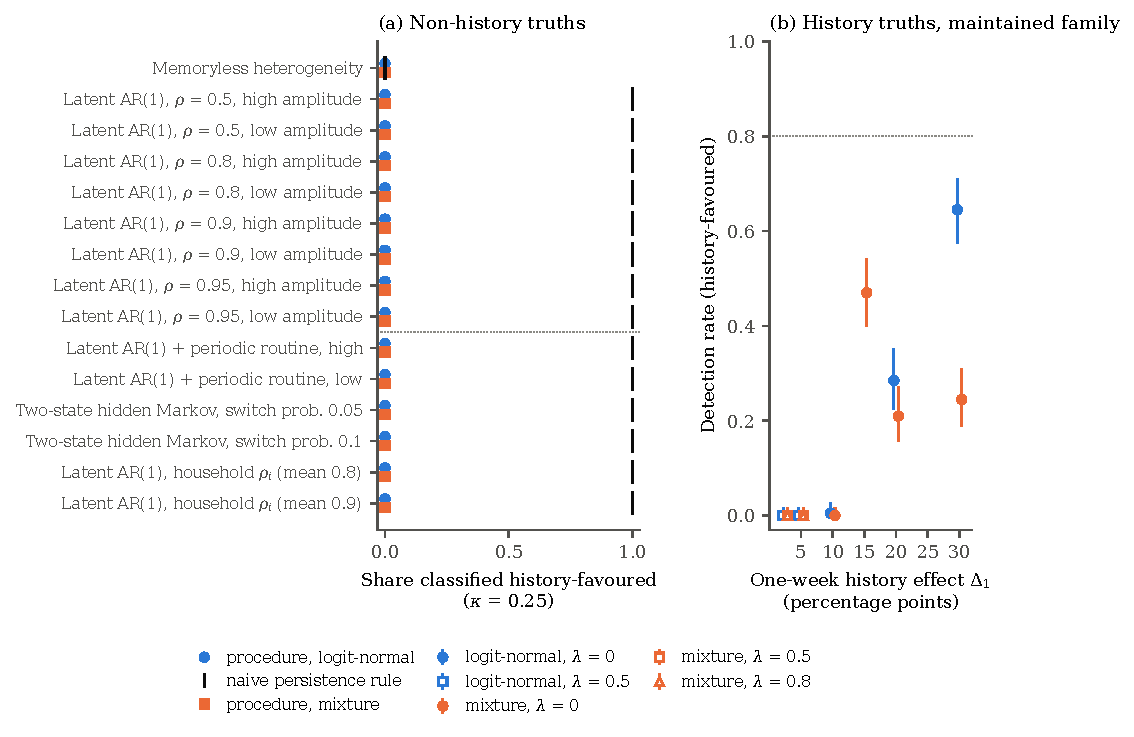
\includegraphics[width=\textwidth]{fig1_known_truth_operating_characteristics.pdf}
\caption{Known truths from the procedure's own families ($\kappa=0.25$; 200 panels per truth;
exact 95 percent intervals). Panel (a): false attribution, for worlds without own-history
dependence. The dotted line separates latent states inside the A1$'$ family from those
outside it, and vertical ticks show the naive rule. Panel (b): detection, for history worlds
of the A2 form, by one-week effect $\Delta_1$ and decay $\lambda$. Truths that could not be
built are omitted: most because the one-week effect is unreachable at that decay, the others
because they could not be calibrated to the real distribution of shopping rates. Rates are
conditional on the common empirical calibration.}
\label{fig:phase8}
\end{figure}

Whether purchase history of the A2 form can mimic a latent state on these five moments
depends on how heterogeneity is specified. The history family could reproduce, within
tolerance, the moments of 4 of the 15 truths without history under logit-normal
heterogeneity, and of 13 under the mixture. Under the mixture, then, history of the A2 form can
mimic almost every history-free world on these moments, and a \verdict{history-favoured}
verdict there depends on the latent family failing clearly.

\subsection{The real panel}

On the real panel, memoryless heterogeneity is inadequate in both specifications. This
confirms, for both forms of heterogeneity, what the positive
within-household coefficient of Section~\ref{sec:data} already suggested. Because the
tolerances are built from what A1 fails to reproduce, the informative evidence is the size of
that failure: the three real lag coefficients and the gain from recent purchases exceed the smallest
discrepancy the procedure can resolve by factors of 4.0 to 7.7, and A1 reproduces essentially
none of them. Those margins are measured in household-bootstrap standard errors, which ignore
shocks common to many households (Section~\ref{sec:limitations}).

Between latent state and purchase history the verdict at the reference tolerance is
\verdict{unresolved} in both specifications, for different reasons. Under logit-normal
heterogeneity the history family is inadequate and the latent family inconclusive. For both,
the binding moment is the share of one-week shopping spells: no parameter point of either
family is shown to reproduce it within tolerance, and at the latent family's closest points
the evidence on that moment is inconclusive rather than clearly outside. Under the mixture,
the latent family is adequate at every tolerance and the history family only at
$\kappa=0.35$, where the comparison becomes \verdict{equivalent}. That mixture result sits at
the design's resolution limit: a finer grid of history parameters, reported as a secondary
analysis, would make the history family adequate at every tolerance and the comparison
\verdict{equivalent}.
\verdict{history-favoured} occurs at none of the three tolerances, in either specification,
or under an alternative observation rule (checked for logit-normal heterogeneity).
Appendix~\ref{app:adequacy} reports the full table.

The real panel therefore does not favor purchase history over a latent state. That is not
evidence that history effects are absent. In-family detection never reached 80 percent at the
reference tolerance, was at most 65 percent even for effects of 15 to 30 points, and was
near zero for effects of 10 points or less, so the unresolved verdict leaves room for history
effects of an economically meaningful size. Under the study's household-bootstrap uncertainty
specification, what the data reject is the simplest explanation,
that persistence reflects stable differences between households of the two tested forms and
nothing else. They do not say which of the two dynamic explanations is right.

% ----------------------------------------------------------------------------
\section{Known truths from learned decision models}
\label{sec:learned}

\subsection{Why test outside the procedure's own families}

Every history truth in Section~\ref{sec:phase8} was generated by A2, the history family the
procedure maintains. The false-attribution test reached partly outside the latent family, but
the detection rates describe only how the procedure behaves when history dependence has
exactly the form it expects. History dependence in real purchasing, if it exists, need not
take that form.

A sharper test needs history mechanisms whose presence or absence is known and whose shape
was not chosen by the analyst. Writing another parametric family would only move the problem,
since it would again be the analyst's family. Randomly drawn response tables would also lie
outside A2, but their shape would come from whatever distribution the analyst drew them from.
The study instead uses existing learned decision models. They respond to recent purchases,
grocery need and shopping frequency through learned response functions that were not specified
by the analyst or by the maintained model families. Each model is asked whether a fully synthetic
household will shop at the store next week and returns a probability, and what it is told is
controlled exactly. Its measured responses then drive simulated panels, and whether
own-history dependence is present is decided by which information the model sees.

None of this treats a learned model as a respondent standing in for a person, which separates the
design from work that uses language models as simulated subjects
\citep{horton2023,argyle2023,aher2023,brand_israeli_ngwe}. A review of generative agent-based
models argues that validation against human data is their central challenge
\citep{larooij2025}, and the same applies to simulated respondents. Simulated subjects also
face treatment variations in the prompt that shift features the analyst did not specify
\citep{gui_toubia}. Here no claim about people is made, every field of the household
description is specified, and paraphrase and placebo controls measure sensitivity to wording.
The closest precedent is in Monte Carlo design. Generative models fitted to real data have been
used to build simulation designs that the researcher did not choose, with a known treatment
effect, for comparing estimators \citep{athey2024}. Pretrained language models have also
supplied the mechanisms of structural causal models whose graph the user specifies, giving
benchmarks with known effects for evaluating treatment-effect estimators \citep{bynum_cho2025}.
Here the learned models are pretrained and not fitted to these data. They supply response
functions the analyst did not choose, the truth is set by what they are shown, and their
measured responses drive a closed-loop dynamic panel, in which each simulated purchase changes
what the model is shown the following week.

\subsection{The learned models and the design}
\label{sec:policies}

The three learned models were neither built nor modified for this study. Each reads a written description of a situation and a yes-or-no question and
returns the probability that the answer is yes. TypeSafe, which develops the first two, calls
models of this kind System One models: they evaluate a natural-language description of a state
and return ``typed answers and probabilities'' rather than generated text
\citep{typesafe_systemone}. Two of the three are pinned versions, 1.13 and 1.14, of TypeSafe's
decision system Jev, both listed as current versioned models \citep{typesafe_models}. The third
is Mercury Decide (Mercury below), a separately developed model from Inception that returns answers with
probabilities in the same way \citep{inception_decisions}. Each version was held fixed
throughout, and every response was checked against the requested version (Appendix~\ref{app:policies}).
Hosted proprietary models can be altered or withdrawn by their providers, which limits the
reproducibility of research that relies on them \citep{palmer2024}, so every simulation in this
section is built from the stored responses rather than from new queries. The two Jev
versions serve as a version-robustness check. A minor version change can alter a learned
system's behavior, so a statement about Jev is made only where both versions agree and is
otherwise reported version by version. The two versions are not independent replications of
each other. Mercury adds a comparison with a separately developed system, but its results are
exploratory, for the reason given at the end of this subsection.

Each query describes a synthetic household by three pieces of information. The first is its
long-run shopping frequency, stated on a ten-level grid from 5 to 95 percent of weeks. The
second is whether it shopped at the store in each of the last four weeks, and the third is its
grocery need in the coming week (less than usual, about usual, or more than usual). History and need are each either shown
or replaced by ``Not provided'', a two-by-two design, and the question asks whether the
household will shop at the store in the coming week. All three models receive the same
information in the same wording, and no household data from the panel are shown to any of
them. Each description was submitted three times to measure repeat noise, once more in a
paraphrase carrying the same information, and, for a stratified sample, with an irrelevant
record number changed as a placebo. An effect counts as interpretable only if it exceeds the
paraphrase effect, the placebo effect and three times the repeat noise, a criterion fixed
before any query was sent.

The measured responses then become a decision rule for simulated households. Each week a
household shops with the model's probability for its current state. Its four-week history
updates from its own purchases, and its need follows a three-state Markov chain. Showing or
hiding history switches own-history dependence on or off, because every model responds to the
history it is shown, and showing or hiding need does the same for a persistent latent state.

To check that the models' behavior stayed stable during data collection, a fixed set of 24
household descriptions was re-queried at four points. The two Jev versions passed this screen.
Mercury triggered it at the third point, after 1,708 of its 3,368 responses, through one
description; a second description also moved materially but stayed within the screen's bound.
Because an analysis of the noise measured before data collection suggested that the screen
would often have stopped a stable model, it was replaced, for Mercury only, by a rule built from
the same measurements, and data collection resumed. Mercury passed the remaining check. The
replacement was chosen after the stop, when both shifts were known, and one element of its
construction decided the outcome: without it, the new rule would also have stopped Mercury at
the third point, through the second shift. Whether the shifts reflect noise or brief drift
cannot be determined from these data. Mercury's results are therefore reported as exploratory,
and the two Jev versions provide the cleanly screened learned-model evidence
(Appendix~\ref{app:policies} gives the details).

\subsection{Controlled responses}

Table~\ref{tab:policies} reports what the models do. In otherwise identical states, showing
that the household shopped last week raises the stated probability of shopping by 13.3, 11.6
and 28.6 percentage points for Jev 1.13, Jev 1.14 and Mercury, and four shopping weeks
against none raise it by 30.6, 28.7 and 65.5. Stating high rather than low need raises it by 11.2 to
52.5 points. Every effect exceeds three standard errors, and the history and need responses
pass the paraphrase, placebo and repeat checks for every model.

\begin{table}[htbp]
\centering\small
\caption{Controlled responses of the three learned models in synthetic states}
\label{tab:policies}
\begin{tabular}{@{}l@{\hspace{14pt}}r@{\,}l@{\hspace{16pt}}r@{\,}l@{\hspace{16pt}}r@{\,}l@{}}
\toprule
 & \multicolumn{2}{c}{Jev 1.13} & \multicolumn{2}{c}{Jev 1.14} & \multicolumn{2}{c}{Mercury} \\
\midrule
\multicolumn{7}{@{}l}{\emph{History}} \\
\quad Last week shopped & 13.32 & (0.10) & 11.56 & (0.10) & 28.55 & (0.20) \\
\quad Average over states visited in simulation & 10.82 & (0.14) & 9.32 & (0.15) & 13.94 & (0.52) \\
\quad Four weeks against none & 30.57 & (0.29) & 28.65 & (0.29) & 65.54 & (0.55) \\
\addlinespace
\multicolumn{7}{@{}l}{\emph{Need high against low}} \\
\quad History hidden & 18.64 & (0.29) & 11.57 & (0.29) & 46.42 & (0.55) \\
\quad History shown & 21.53 & (0.07) & 11.20 & (0.07) & 52.51 & (0.14) \\
\midrule
Paraphrase, placebo and repeat checks & \multicolumn{2}{c}{pass} & \multicolumn{2}{c}{pass} & \multicolumn{2}{c}{pass} \\
Repeat-noise SD & \multicolumn{2}{c}{0.011} & \multicolumn{2}{c}{0.011} & \multicolumn{2}{c}{0.021} \\
Error against stated frequency, no information & \multicolumn{2}{c}{0.031} & \multicolumn{2}{c}{0.036} & \multicolumn{2}{c}{0.197} \\
\bottomrule
\end{tabular}

\smallskip
\parbox{0.92\textwidth}{\footnotesize Percentage points of the model's stated probability of
shopping, with repeat-noise standard errors in parentheses. The average history effect weights
states by how often simulated households driven directly by the model reach them. The last row is the mean absolute gap
between the model's probability and the stated long-run frequency when history and need are
hidden. Mercury's probabilities sit well above the stated frequency (an intercept of about
0.36 when they are regressed on it) and often near 1, and its magnitudes are entangled with that offset and with responses near
the ceiling. Mercury is exploratory (Section~\ref{sec:policies}).
Cross-model differences are not rankings. Measurements of learned models, not of
households.}
\end{table}

Inside the artificial setting these are controlled interventions on the model's input: each
model uses visible history and need. Mercury's larger
numbers partly reflect how far its probabilities sit above the stated frequency, and the two
Jev versions agree in direction almost everywhere while differing in magnitude
(Appendix~\ref{app:policies}).

\subsection{The naive rule on model-driven panels}

When the measured responses drive simulated panels directly, before the anchoring described
below, the naive rule detects every own-history mechanism: its flag rate is 1.00 for all three
models. On panels without own-history dependence, what it does depends on the mechanism and
on the model. With no dynamics it never fires. Some designs show the model \emph{irrelevant
history}: the purchase record of a separately simulated household of the same type, which never
sees the household it is paired with, so it brings in serial structure without any dependence
on the household's own past. When the model reacts to irrelevant history together with latent
need, the rule always fires. When it reacts to irrelevant history alone, the
rate is 0.38, 0.03 and 1.00 for Jev 1.13, Jev 1.14 and Mercury. When it sees only latent need,
whose persistence is set at 0.5, 0.8 and 0.95 in turn, the rate is 0.26, 1.00 and 0.99 for
Jev 1.13, zero throughout for Jev 1.14, and 1 throughout for Mercury. That ordering matches
each model's need response with history hidden (11.6, 18.6 and 46.4 points for Jev 1.14, Jev
1.13 and Mercury), with saturation, although the models differ in several other ways and
three models do not make a dose-response.

Figure~\ref{fig:naive} repeats the exercise on the anchored truths of the next subsection,
whose distribution of shopping rates matches the real panel. Each cell is the share of 200
simulated panels in which the naive rule flags history, with one column per model. The rows
above the line contain no own-history dependence, so every flag there is a false one. They
cover no dynamics at all, and latent need, a persistent need state that the model sees, with
or without the model's history response. They also cover irrelevant history, shown either in
its original order or resampled, with each of the four weeks shown drawn at random, with
replacement, from that household's earlier weeks, which keeps its frequency but removes its
timing. The remaining rows combine latent need with irrelevant history. The rows below the line contain genuine
own history, alone or with latent need. Mercury cells marked with an asterisk were excluded
from the model comparison.

Irrelevant history alone almost never triggers the flag for either Jev version. For Jev 1.13,
irrelevant history in its original order, the design closest to the unanchored one, falls from
0.38 without anchoring to 0.01 with it. Latent need alone triggers the flag for Jev 1.13 (0.89)
and Mercury (1.00) but not for Jev 1.14. For Jev 1.13 the rate rises to 1.00 when the need
response is taken from descriptions with history shown, consistent with its larger need
response there (21.5 against 18.6 points). Latent need together with irrelevant history in its
original order triggers the flag for every model (0.98 to 1.00 across the two heterogeneity
specifications). For Jev 1.14 this joint flag arises although neither input alone crosses the
rule's threshold: the combination is flagged in 0.98 to 0.99 of panels across the two
specifications, against 0.00 for each input alone. Their contributions to the underlying
statistic are roughly additive. Measured against the no-dynamics baseline, latent need adds
0.009 to the two-way lag coefficient, one of the two statistics the rule uses, irrelevant
history adds 0.012, and the two together add 0.024, only 1.3 standard deviations (across
simulated panels) more than the sum of the separate effects.

\begin{figure}[tbp]
\centering
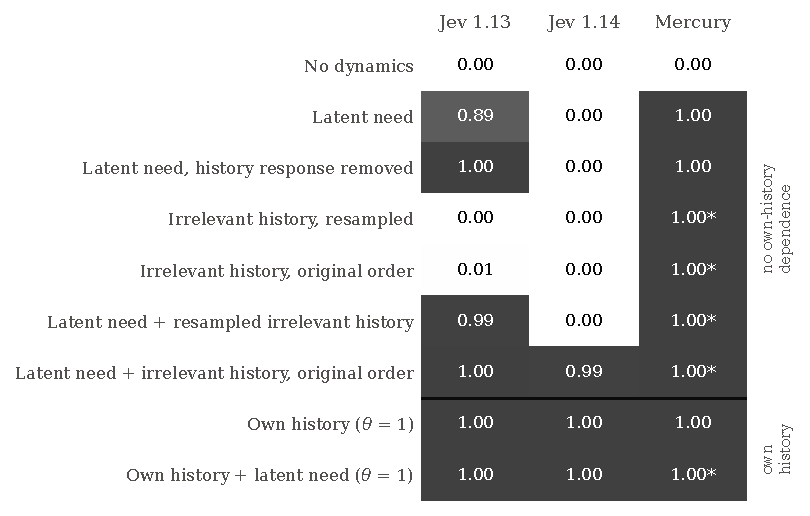
\includegraphics[width=0.82\textwidth]{fig2_naive_flag_by_mechanism.pdf}
\caption{Share of 200 simulated panels flagged by the naive persistence rule, on anchored truths
built from each model's measured responses (logit-normal heterogeneity). Rows above the line
contain no own-history dependence. ``Irrelevant history'' is the purchase record of a separately
simulated household of the same type, shown to the model in its original order or resampled
at random from its earlier weeks. ``History response removed'' keeps the need response measured with history
shown and sets the history response to zero. Rows below the line
contain own-history dependence. An asterisk marks a truth that an admissibility or degeneracy
rule, fixed before any anchored truth was evaluated, excluded from the model comparison.}
\label{fig:naive}
\end{figure}

\subsection{Anchoring}

Without anchoring, the model-driven simulations do not look like the real panel. Every one
of the 93 unanchored variants (31 per model, Appendix~\ref{app:policies}) fails the check on the distribution of shopping rates that every
truth in Section~\ref{sec:phase8} had to pass. The Jev versions compress the distribution, with
too few rare shoppers and too few near-weekly ones, and Mercury shifts it upward. Shifting
every probability by the same amount fixes the mean but not the spread. In a positive control, an idealized
decision rule that returns the stated frequency passes the same check. The finding concerns
only how these three models translate a stated shopping frequency into week-by-week behavior
in this design, and is not a test of how well they model people.

The remedy recalibrates household differences toward the real panel and borrows only the
model's week-to-week response. For each anchored truth the heterogeneity layer of
Section~\ref{sec:framework} is refitted, with the model's dynamics in place, to the real
distribution of shopping rates only, and the truth adds the model's measured response to history and need on the logit scale. For a household
with type level $f_i=\Lambda(\alpha_i)$, four-week purchase record $h_{it}$ and need state
$n_{it}$,
\begin{equation}
\operatorname{logit} p_{it}=\alpha_i+\theta\, g^{H}(h_{it},n_{it}\mid f_i)+g^{N}(n_{it}\mid f_i),
\label{eq:anchored}
\end{equation}
where $\operatorname{logit}(p)=\log[p/(1-p)]$, $g^H$ is the model's history response net of its average over histories, $g^N$ its need
response net of its average over needs, and $\theta\in\{0.25,0.5,0.75,1\}$ scales the history
response (Appendix~\ref{app:anchored}). The construction keeps the analyst's skeleton: the
heterogeneity layer, the logit scale, the four-week window and the need chain. What the model
supplies is the size of the response to every four-week record at every frequency and need
level, and that shape is not the geometric stock of A2.

Fifteen designs per model combine latent need, irrelevant history (in original order or
resampled) and own history at the four values of $\theta$. Three models, fifteen designs and two heterogeneity specifications give 90 truths.
The anchored design was fixed after the unanchored variants had failed, and before any
anchored truth was evaluated.

Anchoring uses only the distribution of shopping rates, which ignores the order of the weeks
within each purchase window.
None of the five dynamic moments enters construction. The anchored truths do share the
heterogeneity layer and the real panel's tolerances with the in-family truths, and the results
are conditional on both. All 30 truths for each Jev version and 16 of 30 for Mercury pass the
admissibility rule and the degeneracy rule, which excludes truths in which more than 5 percent
of simulated probabilities are pushed outside [0.005, 0.995]. That leaves 76 in all: 35 without
own-history dependence and 41 with it. Mercury's 14 exclusions are concentrated in designs that
apply its history response at full or near-full strength, including the irrelevant-history
designs, and in designs that combine history with need, where its probabilities are often near
0 or 1 (Table~\ref{tab:truths}). Its excluded truths have realized one-week effects from 5.2 to 33.8 points (for the
irrelevant-history designs, the visible-history contrast of Table~\ref{tab:outfamily}), so its
contribution below comes from a censored set. One evaluated Mercury truth, own history at full
strength under logit-normal heterogeneity, passes admissibility at its boundary, and its refitted
heterogeneity has almost collapsed (a dispersion of 0.006 on the logit scale), so its spread of
shopping rates comes almost entirely from Mercury's history response. It is kept, as the rules
fixed in advance require.

\subsection{The model comparison out of family}

The design gives the two developers' models different roles. The Jev truths have small
realized one-week own-history effects, $\Delta_1$ of 1.8 to 9.7 points. These are averages over
the states that anchored households actually visit under the real panel's heterogeneity, and
they are smaller than the fixed-state contrasts of Table~\ref{tab:policies} (for Jev 1.13 at
$\theta=1$, 8.96 points realized against a static 13.32). The Jev truths therefore test false attribution and what
the procedure does with effects it would not detect even in family. Mercury, which is
exploratory, is the only model whose realized history effects reach sizes the procedure sometimes
detects in family. Table~\ref{tab:outfamily} and
Figure~\ref{fig:outfamily} give the results.

On every one of the 35 evaluated truths without own-history dependence, including learned
latent need, irrelevant history in either form, and their combinations, the procedure
classified 0 of 200 panels \verdict{history-favoured}, at all three tolerances. The 28 Jev
truths alone give the same result, so it does not depend on Mercury. The
\verdict{latent-favoured} verdicts for Mercury all come from truths with learned latent need,
where the latent family is the closer of the two.

On the 41 evaluated truths with learned own-history dependence, whose one-week effects range
from 1.8 to 26.6 percentage points, the procedure also classified 0 of 200 panels
\verdict{history-favoured}. The verdicts it returned instead differ by model. For the Jev
truths, both families were compatible with the data: \verdict{equivalent} in 73 to 82 percent
of panels and \verdict{unresolved} in most of the rest. Their effects all lie below 10 points,
where in-family detection was already at most 0.005, so they carry little information about
whether the procedure can detect an unfamiliar history mechanism. For Mercury, both families
were inadequate: \verdict{neither} in 79 percent of panels and \verdict{unresolved} in the
rest. Evidence on detection outside the family therefore rests mainly on Mercury's nine
evaluated history truths, which are exploratory.

The Jev versions partly reread the stated shopping frequency from recent history
(Appendix~\ref{app:policies}), as a forecaster inferring a household's type would. In the
simulated world each household's type is fixed, and the learned response is fed back into the
household's probability of shopping the following week, so any response to the household's
own recent purchases is own-history dependence by construction.

\begin{table}[htbp]
\centering\small
\caption{The model-comparison procedure on anchored out-of-family truths}
\label{tab:outfamily}
\setlength{\tabcolsep}{5pt}
\begin{tabular}{@{}l r@{/}l r@{--}l cccc@{}}
\toprule
 & \multicolumn{2}{c}{} & \multicolumn{2}{c}{} & \multicolumn{4}{c}{Share of panels by verdict, $\kappa=0.25$} \\
\cmidrule(l){6-9}
Learned model & \multicolumn{2}{c}{Evaluated} & \multicolumn{2}{c}{Effect range} & Equivalent & Unresolved & Latent & Neither \\
\midrule
\multicolumn{9}{@{}l}{\emph{A. No own-history dependence (correct answer: not history); range of the visible-history contrast}} \\
\quad Jev 1.13 & 14&14 & 0.0&9.6 & 0.986 & 0.014 & --- & --- \\
\quad Jev 1.14 & 14&14 & 0.0&8.6 & 0.990 & 0.010 & --- & --- \\
\quad Mercury  & 7&14  & 0.0&23.6 & 0.571 & 0.260 & 0.169 & --- \\
\addlinespace
\multicolumn{9}{@{}l}{\emph{B. Learned own-history dependence; range of the one-week own-history effect $\Delta_1$}} \\
\quad Jev 1.13 & 16&16 & 2.1&9.7 & 0.820 & 0.176 & 0.004 & --- \\
\quad Jev 1.14 & 16&16 & 1.8&8.6 & 0.727 & 0.273 & --- & --- \\
\quad Mercury  & 9&16  & 5.4&26.6 & --- & 0.208 & --- & 0.792 \\
\bottomrule
\end{tabular}

\smallskip
\parbox{0.94\textwidth}{\footnotesize History-favoured verdicts: 0 of 200 panels in every
evaluated truth in both panels, at $\kappa=0.15$, 0.25 and 0.35 (exact two-sided 95 percent interval
[0, 0.018] per truth). Each truth is one design under one heterogeneity specification, with 200
panels. Evaluated: truths passing the admissibility and degeneracy rules, out of all truths; both rules were fixed before
any anchored truth was evaluated.
Effect range, in percentage points: in panel A, the visible-history contrast, that is, the realized one-week change
in the probability of shopping from switching on the last week of the irrelevant history the
model sees (zero where no irrelevant history is shown), which involves no dependence on the
household's own past purchases. In panel B, the realized one-week own-history effect
$\Delta_1$ of Section~\ref{sec:framework}. Verdict shares are shares of all panels pooled over the evaluated truths, and a dash marks a
verdict that did not occur. The latent-favoured share for Jev 1.13 in panel B is 14 of the 200
panels of one design (own history at full strength with latent need, logit-normal
heterogeneity), a misattribution to the latent family. Mercury results are exploratory and
conditional on the amended stability screen (Section~\ref{sec:policies}).}
\end{table}

\begin{figure}[htbp]
\centering
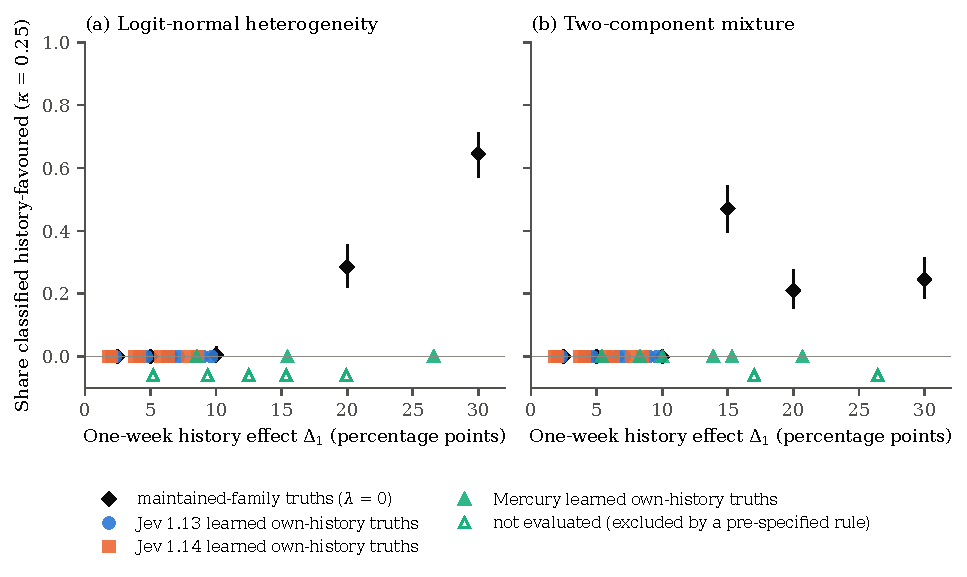
\includegraphics[width=\textwidth]{fig3_in_family_vs_out_of_family.pdf}
\caption{In-family detection against out-of-family learned truths. Black diamonds: share of
panels classified history-favoured for history truths generated by the maintained history family
($\lambda=0$; exact 95 percent intervals). Colored markers: the same share for anchored truths
with learned own-history dependence, all of which are zero. Hollow markers below the axis are
truths excluded by the admissibility or degeneracy rules of Section~\ref{sec:learned}. Mercury
is exploratory (Section~\ref{sec:policies}).}
\label{fig:outfamily}
\end{figure}

Why Mercury's history truths ended in \verdict{neither} is not fully settled. Its history
response differs in shape from the geometric stock of A2 and is larger than the Jev
responses. Three of its nine evaluated history truths also combine latent need with own
history, which no single family represents. In family, the strongest history truths offer no
parallel: at this tolerance they never produced \verdict{neither}, and their misses were
\verdict{unresolved} because the history family was inconclusive (Section~\ref{sec:phase8}).
Which moments failed was not recorded, so these explanations cannot be separated. The implementation itself can return \verdict{history-favoured}: applied to
three stored in-family truths, it reproduces their detection rates exactly (0.645 and 0.285
for the 30- and 20-point truths under logit-normal heterogeneity, 0.470 for the 15-point truth
under the mixture). The procedure names a mechanism
only when that mechanism's family fits, and for these truths neither family did. Taken solely
as a rate of naming history, its record on the learned history truths is therefore the same as
that of a rule that never names history. Among Mercury's truths, \verdict{neither} occurred
only for those with own history, never for those without it. None of the evaluated learned
history mechanisms was attributed to the maintained history family A2. Attribution requires A2
to reproduce the dynamics while the latent family does not, and that combination occurred for
none of these truths.


% ----------------------------------------------------------------------------
\section{Discussion}
\label{sec:discussion}

The two diagnostics make different kinds of mistakes. The naive rule responds to
persistence of every kind: depending on the learned model, it flagged latent need and
irrelevant history as readily as genuine history. The model comparison is conservative by
design, since it asks which family is sufficient for the dynamics. It made no false
attribution in any tested setting, in its own families or outside them, but it detected history
only when the effect was large and of the form it assumed, and it named none of the evaluated
learned history truths.

Every genuine history truth in Section~\ref{sec:phase8} was generated by A2, so the in-family
tests could not show whether the procedure's protection against false attribution, and its
detection, carry over to history whose response shape lies outside that family. The learned
models of Section~\ref{sec:learned} supplied such shapes, which are not the geometric purchase
stock of A2. Out of family, false attribution stayed at zero on
every evaluated truth without own-history dependence. Genuine history of an unfamiliar shape
was never attributed to purchase history: when small, it mostly left both families compatible
with the data, and when larger, in the exploratory Mercury truths, it mostly made both
inadequate. Because the procedure can name history only when its own history family fits, whether
genuine history is attributed depends on the class of models the analyst maintains as well as
on the data. The experiment suggests that this dependence matters in practice, although it cannot
say whether the shape, the size or the combination with need of the learned responses was
responsible in each case.

In the real panel, models in which households differ only in stable shopping rates, in both
forms tested, reproduce essentially none of the within-household dynamics of weekly shopping at
this retailer, while a latent state and purchase history both remain possible. History effects
of 10 points or less would almost certainly not have been found, larger ones only sometimes,
and effects of a different form were not attributed to history at all. For the promotion
question of the Introduction, the data therefore cannot say whether a visit brought about by a
promotion raises the chance of later visits.

The same evidence bears on how persistence is read more generally. In the known-truth worlds,
persistence that survives fixed effects and a predictive gain from recent purchases both arose
from mechanisms in which past purchases have no effect, so neither establishes own-history
dependence on its own. Known-truth simulations measured both of the model comparison's error rates,
which together describe a procedure that avoided false attribution at the cost of limited
detection. Truths from outside the maintained families
showed how far the verdicts depend on those families. The \verdict{unresolved} verdicts in
this paper mark where the data could not separate the two families, and the
\verdict{neither} verdicts mark mechanisms that neither maintained family could reproduce.

The causal section reached a similar position by a different route. There the coupon
regression could be estimated, but without a defensible account of how households were
assigned to campaigns its counterfactual could not be defended. Here a dynamic
coefficient can be estimated, survives household fixed effects and predicts out of sample, and
the mechanism behind it is still not identified. The standard parametric route, a dynamic
random-effects probit with correlated heterogeneity and modeled initial conditions in the
tradition of \citet{heckman1981} and \citet{hyslop1999}, would identify state dependence given
its distributional and exogeneity assumptions. Those assumptions define a maintained class of
exactly the kind whose role this paper measures, and that estimator was not evaluated on the known truths here.
Fixed-effects logit methods \citep{honore_weidner2025} and nonparametric bounds on state
dependence \citep{torgovitsky2019} were not evaluated either. The paper measures the error
rates of one specified attribution procedure and does not benchmark the available estimators of
state dependence.

Several alternatives remain open. Household inventory is the most natural. The timing of
purchases of storable products responds to stocks and prices
\citep{hendel_nevo2006}: a household that stocks up on a product buys it less often
for a while. Regular trip cycles might play a similar role for whole store visits, although
that is a conjecture this analysis does not test. Inventory is itself a form of dependence on
past purchases, but it works through quantities and lowers the chance of buying again soon,
whereas A2 lets past purchases only raise it and A1$'$ has no link to purchases at all.
Modeling inventory needs quantities and prices that this analysis does not use. More
generally, the comparison tests the sufficiency of single-mechanism families in which past
purchases can only raise later shopping. A world with both a latent state and history effects,
or with negative history effects, is judged by whichever single family comes closest, so the
verdicts are not statements about purchase history in general. The families are also compared
on five reduced-form moments only, and estimated dynamic stochastic general equilibrium (DSGE) models in macroeconomics
have met the same difficulty: moments that fit well can still leave the mechanism weakly
identified \citep{canova_sala}.

Credible assignment evidence for the campaigns would reopen the causal question. A history
family flexible enough to span the learned response shapes would show whether Mercury's
\verdict{neither} verdicts reflect the shape of its response or the limits of the two
families, which is a separate research question. More data alone would sharpen the tests without
changing their logic.

\subsection{Limitations}
\label{sec:limitations}

The main empirical evidence covers one retailer and only the decision whether to shop there,
not how much is bought. The real-panel verdicts depend on the heterogeneity specification and, under the
mixture, on the tolerance, and the mixture result sits at the design's resolution limit
(Section~\ref{sec:phase8}). The tolerance floors use household-bootstrap standard errors of the moments under rule $O$,
which do not account for shocks common to many households. No standard error allowing for
common weekly dependence was computed under rule $O$. On the full grid, the Driscoll--Kraay
standard errors of the two-way coefficient are substantially larger than the household- or
two-way clustered ones (Appendix~\ref{app:panel}), so the floors may be too narrow and the
margins reported in Section~\ref{sec:phase8} overstated. Wider floors would make
\verdict{inadequate} verdicts harder to reach and \verdict{equivalent} verdicts easier.

The known-truth rates are conditional on calibrating the simulated families to the real panel,
and the families were not refitted to each simulated panel. Simulated households are independent
and share no common weekly shocks, while in the real panel the week-by-week sums that drive the
regression's standard errors are strongly autocorrelated, so the operating characteristics are
measured for a simpler dependence structure. Admissibility checks only the distribution of
shopping rates, so an admissible history truth can have dynamics unlike the real panel's, and
detection is measured only on admissible truths, which excludes some strong history truths that
distort that distribution, such as the 15-point in-family truth under logit-normal heterogeneity. In family, detection is low at the reference tolerance, partly because of the
resolution of the history family's grid (Section~\ref{sec:phase8}), and long-memory history was
evaluated only at small effects. More
generally, known-truth performance validates a procedure only on the truths it was given
\citep{advani2019}.

The out-of-family evidence uses the heterogeneity layer of Section~\ref{sec:phase8} in its two
specifications, three learned response tables and one construction of truths from them. The Jev
effects are too small to test detection, so evidence on detecting history of an unfamiliar form
rests on Mercury's nine evaluated history truths, which are exploratory because Mercury's data
collection resumed only under a stability screen chosen after the original screen had stopped
it (Section~\ref{sec:policies}). Of Mercury's 30 truths, 14 were excluded,
each a design that applies its history response at full or near-full strength or combines it with
need, and one evaluated truth has almost no fitted stable heterogeneity. The moments responsible for the \verdict{neither} verdicts were not recorded. No
human benchmark exists for the models' magnitudes, which are functions of text measured on
synthetic states.

% ----------------------------------------------------------------------------
\section{Conclusion}
\label{sec:conclusion}

In this panel, 70.8 percent of households that shopped in one week shopped again the next,
compared with 28.5 percent of those that did not. Household fixed effects lower that 42-point
association to 23 points, and adding week effects lowers it to 17. Under the purchase-window
rule $O$, the two-way coefficient is 11 points. Recent
purchases improve the prediction of next week, but a model with no effect of past purchases
gains just as much from them, and the marketing records support no causal design. A model
comparison with rules recorded before its results were computed, though after the real panel's
moments had been examined (Section~\ref{sec:framework}),
rejects, under the study's household-bootstrap uncertainty specification, both tested forms of
stable heterogeneity and leaves latent state against purchase history unresolved. In the simulations it named purchase history in none
of the tested worlds without it, whether they came from its own families or were driven by
learned decision models. At its reference
tolerance it detected large history effects of its own form in at most 65 percent of panels,
and it named none of the evaluated learned ones: for the small Jev effects both families mostly fit,
and for the larger ones of the exploratory Mercury model mostly neither did. These rates are
conditional on calibrating the simulated families to the real panel. Which explanation of persistence one ends up with therefore
depends on which mechanisms one is willing to assume. The data in this panel narrow that set,
by rejecting stable differences alone in both tested forms, but they do not choose within it.

% ----------------------------------------------------------------------------
\section*{AI assistance disclosure}
\addcontentsline{toc}{section}{AI assistance disclosure}

Generative AI tools were used for software implementation and testing under my direction and for
limited editorial assistance. I determined the research questions, research design,
methodological decisions, interpretation of results, and final manuscript content, and I take
responsibility for the work. Separately, learned AI decision models are used as experimental
instruments in the analysis; this use is described in Section~\ref{sec:learned}.

\section*{Data and code availability}

The \emph{Complete Journey} data are distributed by dunnhumby under its own terms and are not
redistributed with this paper. They must be obtained from dunnhumby, which makes the release
available through its source-files page \citep{dunnhumby}. A reproduction package accompanies
the paper. It contains the code, the aggregate results and stored simulation moments behind
every table and figure, a provenance record, checksums, and a single entry point that
checks the reported numbers against their sources, recomputes the known-truth and real-panel
verdicts from the stored moments and, given the \emph{Complete Journey} files, recomputes the
empirical results. The stored model responses are not included while the providers'
redistribution terms are unconfirmed; the package records their checksums, so that an authorized
copy can be verified and the simulations rebuilt from it (Appendix~\ref{app:repro}). The
package is publicly available on GitHub as \texttt{shopping-persistence-reproduction}.\footnote{%
\url{https://github.com/rtmandreyev/shopping-persistence-reproduction}.}

% ----------------------------------------------------------------------------
\begin{thebibliography}{99}
\setlength{\itemsep}{1pt}\small

\bibitem[Advani et~al.(2019)Advani, Kitagawa, and S{\l}oczy{\'n}ski]{advani2019}
Advani, A., T.~Kitagawa and T.~S{\l}oczy{\'n}ski (2019).
Mostly harmless simulations? {U}sing {M}onte {C}arlo studies for estimator selection.
\emph{Journal of Applied Econometrics} 34(6), 893--910.
\href{https://doi.org/10.1002/jae.2724}{doi:10.1002/jae.2724}.

\bibitem[Aher et~al.(2023)Aher, Arriaga, and Kalai]{aher2023}
Aher, G.~V., R.~I. Arriaga and A.~T. Kalai (2023).
Using large language models to simulate multiple humans and replicate human subject studies.
In \emph{Proceedings of the 40th International Conference on Machine Learning}, PMLR 202,
337--371.

\bibitem[Argyle et~al.(2023)Argyle, Busby, Fulda, Gubler, Rytting, and Wingate]{argyle2023}
Argyle, L.~P., E.~C. Busby, N.~Fulda, J.~R. Gubler, C.~Rytting and D.~Wingate (2023).
Out of one, many: Using language models to simulate human samples.
\emph{Political Analysis} 31(3), 337--351.
\href{https://doi.org/10.1017/pan.2023.2}{doi:10.1017/pan.2023.2}.

\bibitem[Athey et~al.(2024)Athey, Imbens, Metzger, and Munro]{athey2024}
Athey, S., G.~W. Imbens, J.~Metzger and E.~Munro (2024).
Using {W}asserstein generative adversarial networks for the design of {M}onte {C}arlo simulations.
\emph{Journal of Econometrics} 240(2), 105076.
\href{https://doi.org/10.1016/j.jeconom.2020.09.013}{doi:10.1016/j.jeconom.2020.09.013}.

\bibitem[Bartolucci et~al.(2018)Bartolucci, Nigro, and Pigini]{bartolucci2018}
Bartolucci, F., V.~Nigro and C.~Pigini (2018).
Testing for state dependence in binary panel data with individual covariates by a modified
quadratic exponential model.
\emph{Econometric Reviews} 37(1), 61--88.
\href{https://doi.org/10.1080/07474938.2015.1060039}{doi:10.1080/07474938.2015.1060039}.

\bibitem[Borusyak et~al.(2024)Borusyak, Jaravel, and Spiess]{borusyak}
Borusyak, K., X.~Jaravel and J.~Spiess (2024).
Revisiting event-study designs: Robust and efficient estimation.
\emph{Review of Economic Studies} 91(6), 3253--3285.
\href{https://doi.org/10.1093/restud/rdae007}{doi:10.1093/restud/rdae007}.

\bibitem[Brand et~al.(2023)Brand, Israeli, and Ngwe]{brand_israeli_ngwe}
Brand, J., A.~Israeli and D.~Ngwe (2023).
Using {LLM}s for market research. SSRN Working Paper 4395751 (originally ``Using GPT for market
research''; revised 2026).
\href{https://doi.org/10.2139/ssrn.4395751}{doi:10.2139/ssrn.4395751}.

\bibitem[Bynum and Cho(2025)]{bynum_cho2025}
Bynum, L.~E.~J. and K.~Cho (2025).
Language models as causal effect generators.
In \emph{Proceedings of the 2025 Conference on Empirical Methods in Natural Language
Processing}, 2096--2115. Association for Computational Linguistics.
\href{https://doi.org/10.18653/v1/2025.emnlp-main.107}{doi:10.18653/v1/2025.emnlp-main.107}.

\bibitem[Callaway and Sant'Anna(2021)]{callaway_santanna}
Callaway, B. and P.~H.~C. Sant'Anna (2021).
Difference-in-differences with multiple time periods.
\emph{Journal of Econometrics} 225(2), 200--230.
\href{https://doi.org/10.1016/j.jeconom.2020.12.001}{doi:10.1016/j.jeconom.2020.12.001}.

\bibitem[Canova and Sala(2009)]{canova_sala}
Canova, F. and L.~Sala (2009).
Back to square one: Identification issues in {DSGE} models.
\emph{Journal of Monetary Economics} 56(4), 431--449.
\href{https://doi.org/10.1016/j.jmoneco.2009.03.014}{doi:10.1016/j.jmoneco.2009.03.014}.

\bibitem[Carrella(2021)]{carrella2021}
Carrella, E. (2021).
No free lunch when estimating simulation parameters.
\emph{Journal of Artificial Societies and Social Simulation} 24(2), 7.
\href{https://doi.org/10.18564/jasss.4572}{doi:10.18564/jasss.4572}.

\bibitem[Chiu et~al.(2026)Chiu, Lan, Liu, and Xu]{chiu2026}
Chiu, A., X.~Lan, Z.~Liu and Y.~Xu (2026).
Causal panel analysis under parallel trends: Lessons from a large reanalysis study.
\emph{American Political Science Review} 120(1), 245--266.
\href{https://doi.org/10.1017/S0003055425000243}{doi:10.1017/S0003055425000243}.

\bibitem[Christensen and Miguel(2018)]{christensen_miguel}
Christensen, G. and E.~Miguel (2018).
Transparency, reproducibility, and the credibility of economics research.
\emph{Journal of Economic Literature} 56(3), 920--980.
\href{https://doi.org/10.1257/jel.20171350}{doi:10.1257/jel.20171350}.

\bibitem[Clopper and Pearson(1934)]{clopper_pearson}
Clopper, C.~J. and E.~S. Pearson (1934).
The use of confidence or fiducial limits illustrated in the case of the binomial.
\emph{Biometrika} 26(4), 404--413.
\href{https://doi.org/10.1093/biomet/26.4.404}{doi:10.1093/biomet/26.4.404}.

\bibitem[de~Chaisemartin and D'Haultf{\oe}uille(2020)]{dechaisemartin}
de~Chaisemartin, C. and X.~D'Haultf{\oe}uille (2020).
Two-way fixed effects estimators with heterogeneous treatment effects.
\emph{American Economic Review} 110(9), 2964--2996.
\href{https://doi.org/10.1257/aer.20181169}{doi:10.1257/aer.20181169}.

\bibitem[Driscoll and Kraay(1998)]{driscoll_kraay}
Driscoll, J.~C. and A.~C. Kraay (1998).
Consistent covariance matrix estimation with spatially dependent panel data.
\emph{Review of Economics and Statistics} 80(4), 549--560.
\href{https://doi.org/10.1162/003465398557825}{doi:10.1162/003465398557825}.

\bibitem[Dub{\'e} et~al.(2010)Dub{\'e}, Hitsch, and Rossi]{dube_hitsch_rossi}
Dub{\'e}, J.-P., G.~J. Hitsch and P.~E. Rossi (2010).
State dependence and alternative explanations for consumer inertia.
\emph{RAND Journal of Economics} 41(3), 417--445.
\href{https://doi.org/10.1111/j.1756-2171.2010.00106.x}{doi:10.1111/j.1756-2171.2010.00106.x}.

\bibitem[dunnhumby(2023)]{dunnhumby}
dunnhumby (2023).
\emph{The Complete Journey User Guide}. Documentation distributed with the \emph{Complete
Journey} data release, \url{https://www.dunnhumby.com/source-files/}.

\bibitem[Fagiolo et~al.(2007)Fagiolo, Moneta, and Windrum]{fagiolo_moneta_windrum}
Fagiolo, G., A.~Moneta and P.~Windrum (2007).
A critical guide to empirical validation of agent-based models in economics: Methodologies,
procedures, and open problems.
\emph{Computational Economics} 30(3), 195--226.
\href{https://doi.org/10.1007/s10614-007-9104-4}{doi:10.1007/s10614-007-9104-4}.

\bibitem[Feller(1943)]{feller1943}
Feller, W. (1943).
On a general class of ``contagious'' distributions.
\emph{Annals of Mathematical Statistics} 14(4), 389--400.
\href{https://doi.org/10.1214/aoms/1177731359}{doi:10.1214/aoms/1177731359}.

\bibitem[Fudenberg et~al.(2022)Fudenberg, Kleinberg, Liang, and Mullainathan]{fudenberg2022}
Fudenberg, D., J.~Kleinberg, A.~Liang and S.~Mullainathan (2022).
Measuring the completeness of economic models.
\emph{Journal of Political Economy} 130(4), 956--990.
\href{https://doi.org/10.1086/718371}{doi:10.1086/718371}.

\bibitem[Gabel et~al.(2026)Gabel, Guhl, Hitsch, and Kook]{gabel2026}
Gabel, S., D.~Guhl, G.~J. Hitsch and K.~H. Kook (2026).
Experimental evidence on structural state dependence in demand.
\emph{Marketing Science}, Articles in Advance, published online 30 October 2026.
\href{https://doi.org/10.1287/mksc.2024.1274}{doi:10.1287/mksc.2024.1274}.

\bibitem[Goodhardt et~al.(1984)Goodhardt, Ehrenberg, and Chatfield]{goodhardt1984}
Goodhardt, G.~J., A.~S.~C. Ehrenberg and C.~Chatfield (1984).
The {D}irichlet: A comprehensive model of buying behaviour.
\emph{Journal of the Royal Statistical Society, Series A} 147(5), 621--655.
\href{https://doi.org/10.2307/2981696}{doi:10.2307/2981696}.

\bibitem[Goodman-Bacon(2021)]{goodman_bacon}
Goodman-Bacon, A. (2021).
Difference-in-differences with variation in treatment timing.
\emph{Journal of Econometrics} 225(2), 254--277.
\href{https://doi.org/10.1016/j.jeconom.2021.03.014}{doi:10.1016/j.jeconom.2021.03.014}.

\bibitem[Grimm et~al.(2005)]{grimm2005}
Grimm, V., E.~Revilla, U.~Berger, F.~Jeltsch, W.~M. Mooij, S.~F. Railsback, H.-H. Thulke,
J.~Weiner, T.~Wiegand and D.~L. DeAngelis (2005).
Pattern-oriented modeling of agent-based complex systems: Lessons from ecology.
\emph{Science} 310(5750), 987--991.
\href{https://doi.org/10.1126/science.1116681}{doi:10.1126/science.1116681}.

\bibitem[Guan et~al.(2018)Guan, Atlas, and Vadiveloo]{guan_atlas_vadiveloo}
Guan, X., S.~A. Atlas and M.~Vadiveloo (2018).
Targeted retail coupons influence category-level food purchases over 2-years.
\emph{International Journal of Behavioral Nutrition and Physical Activity} 15, 111.
\href{https://doi.org/10.1186/s12966-018-0744-7}{doi:10.1186/s12966-018-0744-7}.

\bibitem[Gui and Toubia(2023)]{gui_toubia}
Gui, G. and O.~Toubia (2023).
The challenge of using {LLM}s to simulate human behavior: A causal inference perspective.
arXiv:2312.15524 (revised 2025).
\href{https://doi.org/10.48550/arXiv.2312.15524}{doi:10.48550/arXiv.2312.15524}.

\bibitem[Heckman(1981)]{heckman1981}
Heckman, J.~J. (1981).
Heterogeneity and state dependence.
In S.~Rosen (ed.), \emph{Studies in Labor Markets}, 91--140. University of Chicago Press.
\url{https://www.nber.org/chapters/c8909}.

\bibitem[Hendel and Nevo(2006)]{hendel_nevo2006}
Hendel, I. and A.~Nevo (2006).
Measuring the implications of sales and consumer inventory behavior.
\emph{Econometrica} 74(6), 1637--1673.
\href{https://doi.org/10.1111/j.1468-0262.2006.00721.x}{doi:10.1111/j.1468-0262.2006.00721.x}.

\bibitem[Hnatkovska et~al.(2012)Hnatkovska, Marmer, and Tang]{hnatkovska2012}
Hnatkovska, V., V.~Marmer and Y.~Tang (2012).
Comparison of misspecified calibrated models: The minimum distance approach.
\emph{Journal of Econometrics} 169(1), 131--138.
\href{https://doi.org/10.1016/j.jeconom.2012.01.007}{doi:10.1016/j.jeconom.2012.01.007}.

\bibitem[Honor{\'e} and Kyriazidou(2000)]{honore_kyriazidou}
Honor{\'e}, B.~E. and E.~Kyriazidou (2000).
Panel data discrete choice models with lagged dependent variables.
\emph{Econometrica} 68(4), 839--874.
\href{https://doi.org/10.1111/1468-0262.00139}{doi:10.1111/1468-0262.00139}.

\bibitem[Honor{\'e} and Weidner(2025)]{honore_weidner2025}
Honor{\'e}, B.~E. and M.~Weidner (2025).
Moment conditions for dynamic panel logit models with fixed effects.
\emph{Review of Economic Studies} 92(5), 3112--3137.
\href{https://doi.org/10.1093/restud/rdae097}{doi:10.1093/restud/rdae097}.

\bibitem[Horton(2023)]{horton2023}
Horton, J.~J. (2023).
Large language models as simulated economic agents: What can we learn from homo silicus?
arXiv:2301.07543v1 and NBER Working Paper 31122 (2023); revised 2026 with A.~Filippas and
B.~S. Manning.
\href{https://arxiv.org/abs/2301.07543v1}{arXiv:2301.07543v1}.

\bibitem[Hull(2026)]{hull2026}
Hull, P. (2026).
Two-way fixed effects and modern difference-in-differences: An empirical comparison.
Research note, Brown University, 9 October 2026.
\url{https://github.com/peterdhull/twfe-replication}.

\bibitem[Hyslop(1999)]{hyslop1999}
Hyslop, D.~R. (1999).
State dependence, serial correlation and heterogeneity in intertemporal labor force participation
of married women.
\emph{Econometrica} 67(6), 1255--1294.
\href{https://doi.org/10.1111/1468-0262.00080}{doi:10.1111/1468-0262.00080}.

\bibitem[Imai and Kim(2019)]{imai_kim}
Imai, K. and I.~S. Kim (2019).
When should we use unit fixed effects regression models for causal inference with longitudinal
data?
\emph{American Journal of Political Science} 63(2), 467--490.
\href{https://doi.org/10.1111/ajps.12417}{doi:10.1111/ajps.12417}.

\bibitem[Inception(2026)]{inception_decisions}
Inception (2026).
Decisions. Inception platform documentation.
\url{https://docs.inceptionlabs.ai/capabilities/decisions} (accessed 25 October 2026).

\bibitem[Keane(1997)]{keane1997}
Keane, M.~P. (1997).
Modeling heterogeneity and state dependence in consumer choice behavior.
\emph{Journal of Business \& Economic Statistics} 15(3), 310--327.
\href{https://doi.org/10.1080/07350015.1997.10524709}{doi:10.1080/07350015.1997.10524709}.

\bibitem[Kotschedoff et~al.(2025)Kotschedoff, Kowalczyk, and Breugelmans]{kotschedoff2025}
Kotschedoff, M.~J.~W., L.~Kowalczyk and E.~Breugelmans (2025).
The persistence of grocery shopping behavior and retailer choice: Evidence from a major labor
strike.
\emph{Quantitative Marketing and Economics} 23(3), 447--490.
\href{https://doi.org/10.1007/s11129-025-09298-3}{doi:10.1007/s11129-025-09298-3}.

\bibitem[Larooij and T{\"o}rnberg(2025)]{larooij2025}
Larooij, M. and P.~T{\"o}rnberg (2025).
Validation is the central challenge for generative social simulation: A critical review of {LLM}s
in agent-based modeling.
\emph{Artificial Intelligence Review} 59(1), 15.
\href{https://doi.org/10.1007/s10462-025-11412-6}{doi:10.1007/s10462-025-11412-6}.

\bibitem[Levine and Seiler(2023)]{levine_seiler}
Levine, J. and S.~Seiler (2023).
Identifying state dependence in brand choice: Evidence from hurricanes.
\emph{Marketing Science} 42(5), 934--957.
\href{https://doi.org/10.1287/mksc.2022.1415}{doi:10.1287/mksc.2022.1415}.

\bibitem[McFadden(1989)]{mcfadden1989}
McFadden, D. (1989).
A method of simulated moments for estimation of discrete response models without numerical
integration.
\emph{Econometrica} 57(5), 995--1026.
\href{https://doi.org/10.2307/1913621}{doi:10.2307/1913621}.

\bibitem[Nickell(1981)]{nickell}
Nickell, S. (1981).
Biases in dynamic models with fixed effects.
\emph{Econometrica} 49(6), 1417--1426.
\href{https://doi.org/10.2307/1911408}{doi:10.2307/1911408}.

\bibitem[Olken(2015)]{olken2015}
Olken, B.~A. (2015).
Promises and perils of pre-analysis plans.
\emph{Journal of Economic Perspectives} 29(3), 61--80.
\href{https://doi.org/10.1257/jep.29.3.61}{doi:10.1257/jep.29.3.61}.

\bibitem[OpenRouter(2026)]{openrouter_mercury}
OpenRouter (2026).
Inception: Mercury Decide. Model page.
\url{https://openrouter.ai/inception/mercury-decide} (accessed 25 October 2026).

\bibitem[Pakes and Pollard(1989)]{pakes_pollard}
Pakes, A. and D.~Pollard (1989).
Simulation and the asymptotics of optimization estimators.
\emph{Econometrica} 57(5), 1027--1057.
\href{https://doi.org/10.2307/1913622}{doi:10.2307/1913622}.

\bibitem[Palmer et~al.(2024)Palmer, Smith, and Spirling]{palmer2024}
Palmer, A., N.~A. Smith and A.~Spirling (2024).
Using proprietary language models in academic research requires explicit justification.
\emph{Nature Computational Science} 4(1), 2--3.
\href{https://doi.org/10.1038/s43588-023-00585-1}{doi:10.1038/s43588-023-00585-1}.

\bibitem[Poile and Safayeni(2016)]{poile_safayeni}
Poile, C. and F.~Safayeni (2016).
Using computational modeling for building theory: A double edged sword.
\emph{Journal of Artificial Societies and Social Simulation} 19(3), 8.
\href{https://doi.org/10.18564/jasss.3137}{doi:10.18564/jasss.3137}.

\bibitem[Rambachan and Roth(2023)]{rambachan_roth}
Rambachan, A. and J.~Roth (2023).
A more credible approach to parallel trends.
\emph{Review of Economic Studies} 90(5), 2555--2591.
\href{https://doi.org/10.1093/restud/rdad018}{doi:10.1093/restud/rdad018}.

\bibitem[Roth(2022)]{roth2022}
Roth, J. (2022).
Pretest with caution: Event-study estimates after testing for parallel trends.
\emph{American Economic Review: Insights} 4(3), 305--322.
\href{https://doi.org/10.1257/aeri.20210236}{doi:10.1257/aeri.20210236}.

\bibitem[Roth et~al.(2023)Roth, Sant'Anna, Bilinski, and Poe]{roth_survey}
Roth, J., P.~H.~C. Sant'Anna, A.~Bilinski and J.~Poe (2023).
What's trending in difference-in-differences? {A} synthesis of the recent econometrics literature.
\emph{Journal of Econometrics} 235(2), 2218--2244.
\href{https://doi.org/10.1016/j.jeconom.2023.03.008}{doi:10.1016/j.jeconom.2023.03.008}.

\bibitem[Simonov et~al.(2020)Simonov, Dub{\'e}, Hitsch, and Rossi]{simonov2020}
Simonov, A., J.-P. Dub{\'e}, G.~J. Hitsch and P.~E. Rossi (2020).
State-dependent demand estimation with initial conditions correction.
\emph{Journal of Marketing Research} 57(5), 789--809.
\href{https://doi.org/10.1177/0022243720941529}{doi:10.1177/0022243720941529}.

\bibitem[Sun and Abraham(2021)]{sun_abraham}
Sun, L. and S.~Abraham (2021).
Estimating dynamic treatment effects in event studies with heterogeneous treatment effects.
\emph{Journal of Econometrics} 225(2), 175--199.
\href{https://doi.org/10.1016/j.jeconom.2020.09.006}{doi:10.1016/j.jeconom.2020.09.006}.

\bibitem[Todd and Wolpin(2006)]{todd_wolpin}
Todd, P.~E. and K.~I. Wolpin (2006).
Assessing the impact of a school subsidy program in {M}exico: Using a social experiment to
validate a dynamic behavioral model of child schooling and fertility.
\emph{American Economic Review} 96(5), 1384--1417.
\href{https://doi.org/10.1257/aer.96.5.1384}{doi:10.1257/aer.96.5.1384}.

\bibitem[Torgovitsky(2019)]{torgovitsky2019}
Torgovitsky, A. (2019).
Nonparametric inference on state dependence in unemployment.
\emph{Econometrica} 87(5), 1475--1505.
\href{https://doi.org/10.3982/ECTA14138}{doi:10.3982/ECTA14138}.

\bibitem[TypeSafe(2026a)]{typesafe_systemone}
TypeSafe (2026a).
System One. TypeSafe documentation.
\url{https://docs.typesafe.ai/concepts/system-one} (accessed 25 October 2026).

\bibitem[TypeSafe(2026b)]{typesafe_models}
TypeSafe (2026b).
Models. TypeSafe documentation.
\url{https://docs.typesafe.ai/models} (accessed 25 October 2026).

\bibitem[Vuong(1989)]{vuong1989}
Vuong, Q.~H. (1989).
Likelihood ratio tests for model selection and non-nested hypotheses.
\emph{Econometrica} 57(2), 307--333.
\href{https://doi.org/10.2307/1912557}{doi:10.2307/1912557}.

\end{thebibliography}

% ============================================================================
\clearpage
\appendix
\renewcommand{\thetable}{\thesection.\arabic{table}}
\renewcommand{\thefigure}{\thesection.\arabic{figure}}

\section{Panel persistence: robustness}
\label{app:panel}
\setcounter{table}{0}

\begin{table}[h]
\centering\small
\caption{Robustness of the two-way fixed-effects association}
\label{tab:panel-robust}
\begin{tabular}{@{}l S[table-format=1.3] S[table-format=2.3] S[table-format=1.3]@{}}
\toprule
 & {Participation} & {Revenue} & {Baskets} \\
\midrule
Baseline (responses 2--102, all households) & 0.174 & 11.05 & 0.549 \\
\addlinespace
\emph{Population} & & & \\
\quad $\ge$20 active weeks, active in all thirds (2,115 households) & 0.167 & 10.58 & 0.543 \\
\quad $\ge$30 active weeks, active in all thirds (1,807 households) & 0.170 & 11.09 & 0.581 \\
\addlinespace
\emph{Calendar} & & & \\
\quad Full-week pairs only (responses 3--101) & 0.171 & 10.76 & 0.540 \\
\quad After week 20 (responses 21--101) & 0.103 & 5.19 & 0.337 \\
\addlinespace
\emph{Standard errors of the baseline coefficient} & & & \\
\quad Two-way clustered (household, week) & 0.015 & 1.23 & 0.044 \\
\quad Household clustered & 0.005 & 0.46 & 0.018 \\
\quad Driscoll--Kraay, bandwidth 4 & 0.030 & 2.44 & 0.086 \\
\quad Driscoll--Kraay, bandwidth 8 & 0.038 & 3.11 & 0.111 \\
\addlinespace
\emph{Functional form} & & & \\
\quad $\log(1+\text{revenue})$ & & 0.647 & \\
\bottomrule
\end{tabular}

\smallskip
\parbox{0.94\textwidth}{\footnotesize Coefficients on previous-week participation from
Equation~\eqref{eq:twfe} with household and week effects. Revenue is retailer revenue per
household-week, zeros included. Population and calendar rows use two-way clustered inference, and all
of their 95 percent intervals exclude zero. The log specification changes the outcome and is not an
elasticity. Household clustering ignores cross-household dependence over time and is shown only for
comparison. In the pooled regression the revenue coefficient is 35.01 (1.11), and 14.88 (2.04) with
household effects only.}
\end{table}

Under rule $O$, on the common sample of household-weeks for which all eight lags are
available, the two-way coefficient from regressing participation on a single lag is 0.100,
0.111, 0.096 and 0.061 at lags 1, 2, 4 and 8, and the lag-2 coefficient given lag 1 is 0.102
[0.095, 0.109]. The lag-1 value differs from the 0.112 of Table~\ref{tab:persistence} only
because the sample is smaller. When every household's responses are taken over the
same weeks 20--101, with lags from the full grid, the two-way coefficient is 0.104 [0.095,
0.113]. The regression scores summed
across households are strongly autocorrelated (about 0.96--0.98 at one week and 0.75--0.83 at
eight), which is why Driscoll--Kraay errors are reported.

\section{Purchased composition}
\label{app:composition}
\setcounter{table}{0}

A conditional logit over products would need the set of alternatives on the shelf and their prices
at each purchase occasion. The data show only what was bought, so the analysis narrows to the
National or Private composition of purchases in one sub-commodity, dry spaghetti, chosen from a
screened set before any outcome model was fitted. An event is a basket with positive spaghetti
quantity that is Private-only ($Y_e=1$) or National-only ($Y_e=0$). The 27 mixed baskets are kept in
histories but excluded from the outcome. History uses only events in strictly earlier weeks and is
coded as none recorded (H0), National only (HN, the reference), both (HB) or Private only (HP). The
specification is a linear probability model with store effects and calendar thirds. Household effects
are not included. A conditional fixed-effects logit removes them by conditioning on each household's
number of Private-only events, which requires covariates that do not depend on the household's
outcomes. The history categories are built from its own earlier outcomes, and with such covariates
the household effect can be removed only under additional conditions \citep{honore_kyriazidou}, so
the conditional logit is not a simple solution here.

Among the 6,544 pure events, 22.1 percent are Private-only after a National-only history and
79.2 percent after a Private-only history, and allowing for stores and calendar thirds leaves the
contrast at 53.6 percentage points [49.5, 57.6] (Table~\ref{tab:composition}). The tempting
reading is brand loyalty. But 934 of the 1,560 households are only ever observed in one state, and
a household with a stable taste for private-label spaghetti will have a private-label history and
buy private label now whether or not the history matters. The design describes the gradient but
cannot separate it from stable tastes.

\begin{table}[h]
\centering\small
\caption{Private-only composition of dry-spaghetti baskets by earlier recorded history}
\label{tab:composition}
\begin{tabular}{@{}l r c @{\hspace{18pt}} c c l@{}}
\toprule
 & \multicolumn{2}{c}{Raw} & \multicolumn{3}{c}{Contrast with HN (pp)} \\
\cmidrule(lr){2-3}\cmidrule(l){4-6}
Earlier history & Events & Private-only & No store or third & \multicolumn{2}{c}{Store and third} \\
\midrule
HN: only National & 1,433 & 22.1\% & --- & --- & \\
H0: none recorded & 1,585 & 49.9\% & 29.7 & 27.9 & [22.2, 33.6] \\
HB: both types & 2,064 & 59.6\% & 36.6 & 34.6 & [29.5, 39.8] \\
HP: only Private & 1,462 & 79.2\% & 57.1 & 53.6 & [49.5, 57.6] \\
\bottomrule
\end{tabular}

\smallskip
\parbox{0.94\textwidth}{\footnotesize 6,544 pure events, 1,560 households, 163 stores. Both
contrast columns include history depth $\log(1+n_e)$, where $n_e$ is the number of earlier events, whose coefficient is 1.2 [$-2.5$, 4.8] with
adjustment. Intervals use standard errors clustered by household and week with Student-$t$ (101
degrees of freedom). The full covariance matrix of the store-effects model is not positive
semidefinite, so inference is reported only for the focal coefficients. Of the 1,560 households,
473 are only ever observed Private, 461 only National, and 626 in both states. Descriptive
associations, with persistent household tastes not removed.}
\end{table}

\section{Identification details}
\label{app:did}

\subsection{Guan, Atlas and Vadiveloo (2018)}
The treatment indicator is whether a household received
any of 748 food-related coupons over the two years. In this paper's tabulation of the campaign table,
the 1,584 exposed households are exactly the households ever listed for a campaign, so the object
measured is a listing record rather than observed receipt. The comparison group is the 916 households never listed. The pre-period ends at day
223 and the post-period runs to day 641. Exposed households bought 11.61 items per week before the post
period against 3.08 for the comparison group. No pre-period trend evidence is reported, and a single
aggregated pre-period allows none. The authors acknowledge targeting twice and note that it might bias
their estimates upward.
The five campaigns that start between days 224 and 323 list at most 840 distinct households, and
every other campaign starts on day 346 or later. At least 744 of the 1,584 exposed households
were therefore first listed only in campaigns starting at least 122 days (about seventeen weeks)
after the post period begins. The direction of any resulting bias is not asserted here. Repeated,
overlapping and reversible listings are collapsed into one indicator. None of this demonstrates an
error in their estimate. It shows that its causal reading rests on an undefended counterfactual.

\subsection{Reanalysis evidence}
\citet{chiu2026} reanalyze 49 replicable studies from three political
science journals that use binary-treatment panels. Imputation estimates always share the sign of the
original two-way estimates. Under a relative-magnitude sensitivity bound of $\bar M=0.5$, only 8 of 42
studies still reject a null of no effect. \citet{hull2026}, an unrefereed note released in October 2026,
re-estimates 285 staggered-adoption specifications from 22 studies published in five general-interest
economics journals between 2017 and 2025. In the baseline comparison, estimates change sign in 13.6 and
7.7 percent of pairs for the two newer estimators (pairs include pre-treatment as well as
post-treatment averages), in 1.5 and 1.0 percent of pairs the sign
changes and the difference is statistically significant, and the newer estimators' standard errors are on average
49 and 26 percent larger.

\section{The adequacy rule and the in-family experiment}
\label{app:adequacy}
\setcounter{table}{0}

\subsection{Statistical rule}
Let $d_j$ be the discrepancy for moment $j$ at a parameter point and
$\sigma_{d,j}=\sqrt{SE_j^2+v_j^2/R}$ its standard error, which combines the sampling error $SE_j$ of
the target moment with the Monte Carlo error of $R$ simulated panels whose standard deviation is
$v_j$. Moment $j$ is equivalent if
\[
|d_j|+1.645\,\sigma_{d,j}\le\omega_j
\qquad\text{and clearly outside if}\qquad
|d_j|-2.576\,\sigma_{d,j}>\omega_j,
\]
where 2.576 is the two-tailed Bonferroni critical value for five moments. A point is adequate if all
five moments are equivalent (an intersection--union test of level 0.05) and inadequate if any is
clearly outside (family-wise error at most 0.05). The two cannot both hold. For the real panel
$SE_j$ is the household-bootstrap standard error of the moment under rule $O$. For a known truth
it is the standard deviation of the moment across that truth's 200 panels, as recorded in the
design before any result; the adequacy and verdict rules are otherwise the same.

\subsection{Tolerances}
$E_j$ is the real moment minus the mean of 200 panels from the memoryless
family A1 calibrated to the real cross-sectional distribution. The floor is $\varphi_j=c\,SE_j$ with
$c=4.1598$ for five moments, chosen so that a correctly specified point passes the joint equivalence
test with probability at least 0.80. The constant still carries allowances for the statistical
emulator of the abandoned earlier design (Design history). Under the direct simulation finally
used, the joint pass probability with independent moments is about 0.94, so the floors are wider,
and the rule more conservative, than the 0.80 requirement alone would make them. A moment is resolution-limited when $\varphi_j>\kappa|E_j|$, and
verdicts that rely on such a moment are qualified as holding ``within design resolution''. Because $E_j$
is measured against the logit-normal A1, that family's real-panel $\kappa^*$ is close to 1 by
construction. The evidence that A1 is inadequate is instead that $E_j/\varphi_j$ equals 6.5, 5.1, 7.7 and
4.0 for the three lag coefficients and the gain from recent purchases, and that the mixture version of A1 misses each of them by its full magnitude.

\subsection{Perfect-model checks}
Before it was applied to the real panel, the procedure had to pass five checks
on simulations from correctly specified models, in each heterogeneity specification: the true
parameter in the accepted set in at least 80 percent of panels (observed 0.945--1.000 for
logit-normal heterogeneity and 0.960--1.000 for the mixture), the true family adequate in at least 80
percent (observed at least 0.965), the true family inadequate in at most 5 percent (observed 0), the
true parameter not clearly rejected in at least 90 percent (observed 1), and a memoryless truth
classified history-favoured in at most 10 percent (observed 0). For the history family the only
gate truths that could be built were weak long-memory ones (a one-week effect of 5 points with
$\lambda=0.5$, and also $\lambda=0.8$ under the mixture), so these checks say nothing about the
stronger history truths of Section~\ref{sec:phase8}.

\subsection{Design history}
Two earlier versions of the design were abandoned after failing
their own pre-specified checks, one requiring the two dynamic families to cover comparable
regions of moment space and one testing the accuracy of a statistical emulator for the history
family. Both changes were made before any known-truth result or real-panel adequacy verdict had
been computed, although the real panel's moments had been examined. The mixture specification
was added as a robustness bracket when the design was revised after the first failure. Before
the final design was fixed, simulated values of the five moments at every coarse grid point of
both dynamic families had been committed alongside the tolerances, so with the real moments
known the coarse real-panel comparison was computable; nothing in the record shows that it was
computed or used in choosing the final design, and nothing proves that it was not. The final design simulates every family point directly at its
calibration to the real panel. The simulated truths are not recalibrated one by one, because doing so
for every candidate family and every panel was computationally infeasible. That the known-truth
results were frozen before the real-panel verdict was revealed is documented by time stamps
inside the files and by write-once controls in the code; the two were committed together.

\subsection{Sensitivity to \texorpdfstring{$\kappa$}{kappa}}
At $\kappa=0.35$, logit-normal detection is 0.915 and 0.920 at
$\Delta_1$ of 20 and 30 points, and mixture detection is 0.215, 0.770 and 0.890 at 15, 20 and 30. At
$\kappa=0.15$, logit-normal detection is 0.170 and 0.475 at 20 and 30, and mixture detection is 0.900,
0.110 and 0.035 at 15, 20 and 30. False attribution is zero at every $\kappa$.

\subsection{Truths with both a latent state and history}
Six truths combining an AR(1) state ($\rho=0.9$, high amplitude) with history of the A2 form
($\lambda=0.5$), at one-week effects of 2.5 to 30 points, were specified in advance with the other
truths but are not part of the summary in Section~\ref{sec:phase8}. Only those at 10 points or
less could be built. At $\kappa=0.25$, under logit-normal heterogeneity, they were classified
\verdict{latent-favoured} in 200 and 197 of 200 panels at 2.5 and 5 points, and at 10 points
\verdict{neither} in 34 and \verdict{unresolved} in 166. Under the mixture they were
\verdict{equivalent} or \verdict{unresolved}, except at 10 points, where 1 of 200 panels was
classified \verdict{history-favoured} (11 at $\kappa=0.15$). A combination of a latent state with
modest history is therefore mostly attributed to the latent family or left undecided.

\subsection{Post hoc diagnostic: detection and grid resolution}
The diagnostic below was run after an independent audit of the repository, to examine the
non-monotone detection reported in Section~\ref{sec:phase8}. It uses the stored panels, involves
no new simulation and is not part of the recorded design. Each dynamic family was evaluated at every grid point already
simulated (the coarse lattice and all precomputed first-level refinement points) instead of at
the refinement points the recorded rule selects; the verdict rules were unchanged. At
$\kappa=0.25$, detection of the 20-point truths rises from 57 to 198 of 200 panels under
logit-normal heterogeneity and from 42 to 200 under the mixture. The 30-point truths are unchanged
(129 and 49 of 200), the 15-point truth under the mixture falls from 94 to 86, and no history-free
truth is classified \verdict{history-favoured} at any tolerance. The 20-point truths lie midway
between two grid values of $\delta$, next to an already-simulated refinement point that the
recorded rule rarely selects, so their low recorded detection is largely a limit of the grid's
resolution. For the 30-point truths, evaluating every simulated point does not help, and the
stored outputs cannot show whether a finer grid would. The diagnostic changes no reported rate.

\begin{table}[h]
\centering\small
\caption{Real-panel adequacy by heterogeneity specification}
\label{tab:real}
\begin{tabular}{@{}l l l c c@{}}
\toprule
Specification & Family & Verdict at $\kappa=0.25$ (comparison at three $\kappa$) & $\kappa^*$ & Binding moment \\
\midrule
Logit-normal & A1 & inadequate & & \\
             & A1$'$ (latent) & inconclusive & 1.179 & one-week spells \\
             & A2 (history) & inadequate & 1.340 & one-week spells \\
             & A1$'$ vs A2 & \textsc{unr} / \textsc{unr} / \textsc{unr} at $\kappa$ = 0.15 / 0.25 / 0.35 & & \\
\addlinespace[6pt]
Mixture      & A1 & inadequate & & \\
             & A1$'$ (latent) & adequate & 0.000 & none \\
             & A2 (history) & inconclusive; adequate at 0.35 & 0.252 & lag-8 \\
             & A1$'$ vs A2 & \textsc{unr} / \textsc{unr} / \textsc{eq} at $\kappa$ = 0.15 / 0.25 / 0.35 & & \\
\bottomrule
\end{tabular}

\smallskip
\parbox{0.94\textwidth}{\footnotesize $\kappa^*$ is the smallest tolerance multiple, possibly
outside the tested range, at which the family would become adequate (0 when it meets every tolerance floor), and the moment that binds it; no moment binds when $\kappa^*=0$.
A family can be inadequate at every tested $\kappa$ and still have a finite $\kappa^*$. Mixture
adequacy holds within design resolution. Under an alternative observation rule (logit-normal),
in which each simulated household can shop only between a first and last week drawn from the
real households' purchase windows, the comparison is \textsc{unresolved} at every $\kappa$. A finer grid,
reported as secondary, would make the mixture version of A2 adequate at every $\kappa$, so the
mixture verdict at 0.25 sits at the design's resolution limit. \textsc{unr}:
unresolved; \textsc{eq}: equivalent.}
\end{table}

\section{The learned decision models}
\label{app:policies}

\subsection{Models and data collection}
The models are \texttt{jev-1.13.0} and
\texttt{jev-1.14.0}, developed by TypeSafe and queried through its own interface, and
\texttt{inception/mercury-decide-20260930}, developed by Inception and queried through
OpenRouter, which lists it as a System One model \citep{openrouter_mercury}, with Inception as the
only provider. Every response was checked against the
requested version, and versions were never mixed. Each model, Mercury included, answered the
same complete set of 3,368 queries in October 2026. All responses were stored, and every
simulation in the paper is built from the stored responses.

\subsection{Wording}
The main template states, for example: ``Over the long run, this household shops at
this grocery store in about 35\% of weeks''; ``Last week: shopped at this grocery store. 2 weeks ago: did
not shop at this grocery store\ldots''; ``Shopped at this grocery store in 2 of the last 4 weeks''; ``In
the coming week, the household needs more groceries than usual''; and ``Record ID 4821''. The question is
``Will this household shop at this grocery store in the coming week?'', with explicit true and false
criteria. Each query also asks the complementary question (no purchase) and whether the household
shops in most weeks over the long run, a negative-control outcome. The paraphrase template changes every
sentence while preserving content and numeric format, and the placebo changes the record identifier to 7356.
History summaries are computed from the four-week record, so no inconsistent state can be shown.

\subsection{State space and validity}
With ten frequency levels, the state space has 10 states with
neither history nor need shown, 30 with need only, 160 with history only and 480 with both. An effect is
labeled positive or negative when its magnitude exceeds three repeat-noise standard errors. The history
and need responses count as interpretable only if each paired effect exceeds paraphrase sensitivity and
placebo sensitivity (one-sided 95 percent stratified bootstrap lower bound above zero) and three times
the repeat noise. Every effect in Table~\ref{tab:policies} is labeled positive whether the probability of
shopping or the normalized probability shop/(shop + skip) is used. On the
negative-control question, whether the household shops in most weeks, showing recent history
moves both Jev versions' answers but not Mercury's: the Jev versions partly reread stated type
from history.

\subsection{Information interactions and cross-model comparisons}
Stating the long-run shopping frequency reduces the
history effect for every model (8.18, 10.11 and 2.73 points). Stating need lowers it by 2.10
points for Mercury (standard error 0.23) and raises it by 1.04 points for Jev 1.14 (0.12); for
Jev 1.13 the change, 0.18 points (0.12), is not distinguishable from zero, so no general direction
is claimed. The stored inventory of 65 labels covers the effect and validity labels, each also
under the normalized probability, and the admissibility labels of the unanchored truths; the two
Jev versions give the same label on 63 of them, and the two exceptions are the need interaction
under both probability conventions. Their need effects are 18.6 and 11.6 points and their one-week
history effects differ by about 12 standard errors. Jev and Mercury agree on 63 labels, disagree on none,
and two are not comparable because the Jev label differs between versions. Outside that inventory
Mercury differs: an upward intercept of about 0.36 (error against the stated frequency 0.197), twice the
repeat noise, discrete answers, and magnitude ratios of 2 to 2.5 for the one-week and four-week history
effects and 2.4 to 4.7 for need.

\subsection{Simulation checks}
For every design in which the model sees no other household's history, analytic and simulated rates
and joint transition probabilities agree within 0.005, and the total variation distance from the stationary distribution after the 26-week burn-in is
at most $4.6\times10^{-3}$. The unanchored simulations use each model's response table in up to three versions: as
measured, with a single shift applied to all of its logits so that the simulated mean shopping
rate matches the real panel's, and as a logistic approximation fitted to the table. Seven of the
12 closed-loop designs use all three, and the five with irrelevant history or no dynamics use the
first two, which gives the 31 variants per model of Section~\ref{sec:learned}. The shift ranges
from $-0.07$ to $+0.22$ for Jev and from $-1.0$ to $-1.9$ for Mercury.

\subsection{Stability monitoring and the Mercury amendment}
Twenty-four sentinel states (12 with
history and need both shown, 6 with history only, 3 with need only and 3 with neither) were re-queried at
four time points. The original screen, specified before data collection, stopped a run if the median shift
exceeded $\max(0.02,3\sigma)$ or any single sentinel moved more than $\max(0.10,6\sigma)$, with $\sigma$
the repeat noise pooled across four test states measured before data collection (0.027 for
Mercury, a different quantity from the repeat-noise SD of the full query set in
Table~\ref{tab:policies}). Mercury's data collection stopped at the third time point, after 1,708 of its responses: one sentinel moved from 0.651
to 0.469, a shift of 0.183 against a bound of 0.164, while the median shift was 0.0007. A second
sentinel, with history only, moved from 0.407 to 0.294, a shift of 0.113 that was inside the
original bound. Both sentinels describe a household stated to shop in 95 percent of weeks with no
recent purchase, both moved down, and both partly reverted by the fourth time point.

Two features of the original screen may have given it a high false-stop probability. The pooled $\sigma$ gave the sentinels in the both-shown
cell, half of all sentinels, a quarter of the weight, while that cell's measured noise was 0.050. And the
single-shift rule took a maximum over 72 comparisons without family-wise calibration. Simulating the
original screen for a stable Mercury, using only the pre-collection noise measurements and the fixed
sentinel composition, gives a false-stop probability of 0.37 by the third time point and 0.49 by
the fourth when each cell's own measured noise is used, but about 0.001 when a single pooled noise
level is used, and anywhere from about 0.003 to about 1 across the uncertainty interval of the
both-shown noise; the size of the miscalibration is therefore poorly determined. The 24 sentinels
showed no common directional movement, and the reported model and provider did not change. The
two shifts are consistent both with noise in a poorly measured cell and with brief drift in
those states, and the data cannot distinguish the two. Drift was neither established nor ruled
out.

After the stop, the screen was replaced for Mercury only by a cell-stratified rule calibrated to a 1
percent family-wise false-stop rate: $b_c=\max(0.10,\,3.80\sqrt2\,\sigma_c)$ with
$\sigma_c=\max(\sigma_{c,\text{pre}},\sigma_{\text{pooled}})$, giving bounds of 0.269 for the
both-shown cell and 0.147 elsewhere, with the median rule unchanged. The new rule's inputs were
the pre-collection noise measurements only, but its construction was chosen after the stop, when
both third-point shifts were known, so it is not prospective. One element of that construction
decided the outcome. The floor $\sigma_{\text{pooled}}$ raises the bound for the history-only cell
from 0.10 to 0.147; without it, the same stratified rule would have stopped Mercury at the third
time point, through the history-only shift of 0.113, at the same point as the original screen. The
floor's stated purpose, keeping cells with zero measured noise from shrinking a bound, is already
served by the minimum of 0.10. Data collection resumed, and Mercury passed the fourth check. All
3,368 Mercury responses are used in every Mercury estimate: 1,708 collected before the stop and
1,660 after the amendment. The pre-stop responses alone leave 99 of the 748 descriptions without
any answer and give all three repeats for only 89, so no Mercury analysis in this paper can be
computed from them alone. For these reasons Mercury's results are reported as exploratory. Under the original
screen alone, Mercury would have been excluded, although the shift that triggered the stop lies inside
the amended bound. Under the amended rule, a stop at the fourth check would have removed Mercury from the
study permanently. The amended rule needs a
single both-shown sentinel to move by about 0.27 before it stops, and with five pre-collection draws per
state the both-shown $\sigma$ is poorly identified (95 percent interval 0.030 to 0.144), so the screen's
sensitivity to drift in that cell is weak. The two Jev runs passed the original screen, with a largest
sentinel shift of 0.05.

\section{Anchored truths}
\label{app:anchored}
\setcounter{table}{0}

Let $\pi(h,n;f)$ be a model's measured probability for four-week record $h$, need $n$ and
stated frequency $f$, clipped to [0.005, 0.995], and let $w(h;f)$ be the Binomial$(4,f)$
probability of record $h$. Then
\[
g^H(h,n\mid f)=\operatorname{logit}\pi(h,n;f)-\sum_{h'}w(h';f)\operatorname{logit}\pi(h',n;f),
\]
and $g^N(n\mid f)$ is the history-averaged term $\sum_{h'}w(h';f)\operatorname{logit}\pi(h',n;f)$
minus its average over need levels. A household's type
coordinate is $f_i=\Lambda(\alpha_i)$ restricted to [0.05, 0.95], and both parts are interpolated linearly
between grid levels. The need chain is symmetric with three states and persistence 0.8. Irrelevant history comes from a shadow household simulated alongside each household: it has the
same type $\alpha_i$, evolves under the same dynamics on its own history and need, and never
sees the household it is paired with, so households remain independent and no household's own
purchases reach the history its model is shown. Irrelevant history in original order is the
shadow's realized purchases in the previous four weeks. Resampled irrelevant history draws each
of the four positions independently and with replacement from the shadow's purchases in all
earlier weeks, keeping its running frequency and removing its order. A truth is \textsc{degenerate} if more than 5 percent of
household-weeks after burn-in have probabilities outside [0.005, 0.995], and \textsc{infeasible} if its
calibrated population fails the cross-sectional check. Both are reported and never adjusted.
For each truth the heterogeneity layer, $(\mu,s)$ or the mixture parameters, is refitted to the
real distribution of shopping rates with the model's dynamics in place, and the cross-sectional
check is then repeated on a separate block of 200 simulated panels.

\begin{table}[h]
\centering\small
\caption{The fifteen anchored designs per model and heterogeneity specification}
\label{tab:truths}
\begin{tabular}{llll}
\toprule
Design & History input to the model & Latent need & $\theta$ \\
\midrule
N1 & none & none & --- \\
N2 & none & yes & --- \\
N3, N4 & irrelevant history, resampled / original order & none & 1 \\
N5, N6 & irrelevant history, resampled / original order & yes & 1 \\
N7 & none (history response removed) & yes & 0 \\
H1--H4 & own history & none & 0.25, 0.5, 0.75, 1 \\
H5--H8 & own history & yes & 0.25, 0.5, 0.75, 1 \\
\bottomrule
\end{tabular}

\smallskip
\parbox{0.94\textwidth}{\footnotesize N1--N7 contain no own-history dependence, and H1--H8 contain it. The 14
excluded Mercury truths are, under logit-normal heterogeneity, N3 and N4 (infeasible), N5, N6, H5, H6, H7
and H8 (infeasible and degenerate) and H3 (infeasible); under the mixture, N3, N4 and H4 (infeasible) and
N6 and H8 (degenerate). Their realized one-week effects (the visible-history contrast for N
designs, $\Delta_1$ for H designs) run from 5.2 to 33.8 points.}
\end{table}

\FloatBarrier
\section{Reproducibility}
\label{app:repro}

The analysis was governed by versioned decision records, written stage by stage before each
stage was run, and every later change of design is recorded with its reason. Four deviations from
a fully prospective design bear on the results. The families, moments, tolerances and verdict
rules were fixed after the real panel's values of the calibration target and the five moments had
been examined, though before any known-truth result or real-panel adequacy verdict was computed
(Section~\ref{sec:framework}). Two earlier versions of the in-family design were abandoned after
failing their own checks, also before any known-truth result or real-panel adequacy verdict;
the mixture specification was added at that stage, and simulated moments for every coarse grid
point were committed before the final design was fixed (Appendix~\ref{app:adequacy}). Anchoring was adopted after every unanchored model-driven truth
had failed the admissibility check, and was fixed before any anchored truth was evaluated
(Section~\ref{sec:learned}). Mercury's stability screen was replaced after it stopped data
collection, by a rule whose construction was chosen with the stop's outcome known, so Mercury's
results are exploratory (Appendix~\ref{app:policies}). The grid-resolution diagnostic in
Appendix~\ref{app:adequacy} was run after an independent audit of the repository and is not part
of the recorded design. The stored model responses allow
every simulation to be rebuilt without querying the models again, and the figures are drawn
directly from the recorded results without recomputation. The public reproduction package,
\texttt{shopping-persistence-reproduction} (Data and code availability), verifies the reported numbers, recomputes the known-truth and real-panel verdicts
from the stored simulation moments, recomputes the empirical results from the raw files and,
from an authorized copy of the stored responses, reruns the learned-model simulations. The
original model queries cannot be repeated exactly, and the known-truth production run (about 200
core-hours) is not rerun. The \emph{Complete Journey} data must be obtained from dunnhumby.

\end{document}
